% Paquets généraux
\documentclass[a4paper,12pt,titlepage,twoside]{article}
\usepackage[T1]{fontenc}
\usepackage[utf8]{inputenc}
\usepackage[french]{babel}
\usepackage{subcaption}
\addto\captionsfrench{%
  \renewcommand{\tablename}{Tableau}%
}
\usepackage[gen]{eurosym}
%\usepackage[dvips]{graphicx}
\usepackage{minted}
\usepackage{fancyhdr}
\usepackage{pdfpages} 
\usepackage{multido}
\usepackage{hyperref}
\usepackage{textcomp}
\usepackage{schemabloc}
%\usepackage[bitstream-charter]{mathdesign}
\usepackage{array}
\newcolumntype{P}[1]{>{\centering\arraybackslash}p{#1}}
\usepackage[shortlabels]{enumitem}
\usepackage[framemethod=TikZ]{mdframed}

\newcommand{\id}{71}
\newcommand{\nom}{Théorie des mécanismes}
\newcommand{\sequence}{04}
\newcommand{\nomsequence}{Liaisons entre les solides}
\newcommand{\num}{02}
\newcommand{\type}{KH}
\newcommand{\descrip}{Liaisons équivalentes, hyperstatisme, liaisons en série et en parallèle, théorie des graphes}
\newcommand{\competences}{B2-12: Proposer une modélisation des liaisons avec leurs caractéristiques géométriques. \\ &  B2-13: Proposer un modèle cinématique paramétré à partir d'un système réel, d'une maquette numérique ou d'u \\ &  B2-17: Simplifier un modèle de mécanisme. \\ &  B2-18: Modifier un modèle pour le rendre isostatique. \\ &  C1-04: Proposer une démarche permettant d'obtenir une loi entrée-sortie géométrique.  \\ &  C2-05: Caractériser le mouvement d'un repère par rapport à un autre repère. \\ &  C2-06: Déterminer les relations entre les grandeurs géométriques ou cinématiques. }
\newcommand{\nbcomp}{7}
\newcommand{\systemes}{}
\newcommand{\systemesnum}{}
\newcommand{\systemessansaccent}{}
\newcommand{\ilot}{2}
\newcommand{\ilotstr}{02}
\newcommand{\dossierilot}{\detokenize{Ilot_02 }}

%\usepackage{style}
\usepackage{bodegraph}
\usepackage{rpcinematik}
\usepackage[locale = FR]{siunitx}
\usepackage{caption}
\newcommand{\institute}{Lycée Dorian}

\usepackage{listings}
\usepackage{fancyvrb}
\usepackage{color}
\usepackage{xcolor}
\usepackage{colortbl}
\usepackage{helvet}
\usepackage[frenchmath]{newtxsf} % for sans serif symbols
\renewcommand{\familydefault}{\sfdefault}
%\usepackage{amsfonts}
%\usepackage{amsmath}
%\usepackage{lmodern}
\usepackage{mathastext}
%\usepackage{xspace}
\usepackage{varioref}
\usepackage{tabularx}
%\usepackage{floatflt}
\usepackage{graphics}
\usepackage{wrapfig}
\usepackage{textcomp}
\usepackage{tikz,tkz-tab}
\usepackage[european resistor, european voltage, european current]{circuitikz}
\usepackage{wrapfig}
\usepackage{gensymb}
\usepackage[percent]{overpic}
\usetikzlibrary{babel}
\usepackage{ifthen}
\usepackage{cancel}
\usepackage{etoolbox}
\usepackage{multirow}
%\usepackage{boxedminipage}
\definecolor{gris25}{gray}{0.75}
\definecolor{bleu}{RGB}{18,33,98}
\definecolor{bleuf}{RGB}{42,94,171}
\definecolor{bleuc}{RGB}{231,239,247}
\definecolor{bleum}{RGB}{160,195,226}
\definecolor{rougef}{RGB}{185,18,27}
\definecolor{rougec}{RGB}{255,188,204}%255,230,231
\definecolor{vertf}{RGB}{103,126,82}
\definecolor{vertc}{RGB}{220,255,191}
\definecolor{forestgreen}{rgb}{0.13,0.54,0.13}
\definecolor{blcr}{rgb}{0.59,0.69,0.84}
\definecolor{blfr}{rgb}{0.32,0.51,0.75}
\definecolor{orfr}{rgb}{0.90,0.42,0.15}
\definecolor{orcr}{rgb}{0.90,0.65,0.50}
\definecolor{orangef}{rgb}{0.659,0.269,0.072}
\definecolor{orange}{rgb}{0.58,0.35,0.063}
\definecolor{orangec}{rgb}{0.43,0.32,0.25}
\definecolor{rcorrect}{rgb}{0.6,0,0}
\definecolor{sequence}{rgb}{0.75,0.75,0.75}
\definecolor{competences}{rgb}{0.61,0.73,0.35}
\definecolor{rose}{HTML}{ff00ff}
\definecolor{grisf}{HTML}{222222}
\definecolor{grisc}{HTML}{636363}
\definecolor{normal}{HTML}{4087c4}
\definecolor{info}{HTML}{5bc0de}
\definecolor{success}{RGB}{92,184,92}
\definecolor{warning}{RGB}{240,173,78}
\definecolor{danger}{RGB}{217,83,79}
\hypersetup{                    % parametrage des hyperliens
    colorlinks=true,                % colorise les liens
    breaklinks=true,                % permet les retours à la ligne pour les liens trop longs
    urlcolor= blfr,                 % couleur des hyperliens
    linkcolor= orange,                % couleur des liens internes aux documents (index, figures, tableaux, equations,...)
    citecolor= forestgreen                % couleur des liens vers les references bibliographiques
    }

\newcolumntype{M}[1]{>{\centering\arraybackslash}m{#1}}
\definecolor{codegreen}{rgb}{0,0.6,0}
\definecolor{codegray}{rgb}{0.5,0.5,0.5}
\definecolor{codepurple}{rgb}{0.58,0,0.82}
\definecolor{backcolour}{rgb}{0.95,0.95,0.92}

\lstdefinestyle{mystyle}{
    backgroundcolor=\color{backcolour},   
    commentstyle=\color{codegreen},
    keywordstyle=\color{magenta},
    numberstyle=\tiny\color{codegray},
    stringstyle=\color{codepurple},
    basicstyle=\ttfamily\footnotesize,
    breakatwhitespace=false,         
    breaklines=true,                 
    captionpos=b,                    
    keepspaces=true,                 
    numbers=left,                    
    numbersep=5pt,                  
    showspaces=false,                
    showstringspaces=false,
    showtabs=false,                  
    tabsize=2
}

\lstset{style=mystyle}

% Mise en page
\pagestyle{fancy}

\setlength{\hoffset}{-18pt}
\setlength{\oddsidemargin}{0pt} 	% Marge gauche sur pages impaire2s
\setlength{\evensidemargin}{0pt} 	% Marge gauche sur pages paires
\setlength{\marginparwidth}{00pt} 	% Largeur de note dans la marge
\setlength{\headwidth}{481pt} 	 	% Largeur de la zone de tête (17cm)
\setlength{\textwidth}{481pt} 	 	% Largeu\textbf{r de la zone de texte (17cm)
\setlength{\voffset}{-18pt} 		% Bon pour DOS
\setlength{\marginparsep}{7pt}	 	% Séparation de la marge
\setlength{\topmargin}{-30pt} 		% Pas de marge en haut
\setlength{\headheight}{55pt} 		% Haut de page
\setlength{\headsep}{20pt} 		% Entre le haut de page et le texte
\setlength{\footskip}{30pt} 		% Bas de\textbf{ page + séparation
\setlength{\textheight}{700pt} 		% Hauteur de l'icone zone de texte (25cm)
\setlength\fboxrule{1 pt}
\renewcommand{\baselinestretch}{1}
\setcounter{tocdepth}{1}
\newcommand{\cadre}[2]
{\fbox{
  \begin{minipage}{#1\linewidth}
   \begin{center}
    #2\\
   \end{center}
  \end{minipage}
 }
}

\newcommand{\repon}[1]
{
~\ \\
\begin{tabular}{|m{\linewidth}|}
 \hline
\multido{}{#1}{\\ \hline}
\end{tabular}
}


\newcommand{\objectif}[1]{
\mdfsetup{%
frametitle={%
\tikz[baseline=(current bounding box.east),outer sep=0pt]
\node[anchor=east,rectangle,fill=bleum]
{\strut Objectif~};}}
\mdfsetup{innertopmargin=10pt,linecolor=bleum,%
linewidth=2pt,topline=true,%
frametitleaboveskip=\dimexpr-\ht\strutbox\relax
}
\begin{mdframed}[]\relax%
#1
\end{mdframed}}


\newcounter{num_quest} \setcounter{num_quest}{0}
\newcounter{num_rep} \setcounter{num_rep}{0}
\newcounter{num_cor} \setcounter{num_cor}{0}

\newcommand{\feuilleDR}[1]{
	\begin{tikzpicture}
		\draw[gray!30](0,0)grid[step=0.5cm](\linewidth,#1);
	\end{tikzpicture}
}

%\newcommand{\question}[1]{\refstepcounter{num_quest}\par
%~\ \\ \parbox[t][][t]{0.15\linewidth}{\textbf{Question \arabic{num_quest}}}\parbox[t][][t]{0.85\linewidth}{#1\label{q\the\value{num_quest}}}\par
%}

\newcommand{\question}[1]{\refstepcounter{num_quest}\par
~\ \\ \textbf{Question \arabic{num_quest} : }#1\label{q\the\value{num_quest}}\par
}

\newcommand{\posetafigure}[3]{
\begin{figure}[ht!]
 \begin{center}
  \includegraphics[width=#2\linewidth]{img/#1}
 \end{center}
 \caption{\label{#1} #3}
\end{figure}}

\newcommand{\goforum}{
\begin{figure}

\end{figure}
\begin{center}
 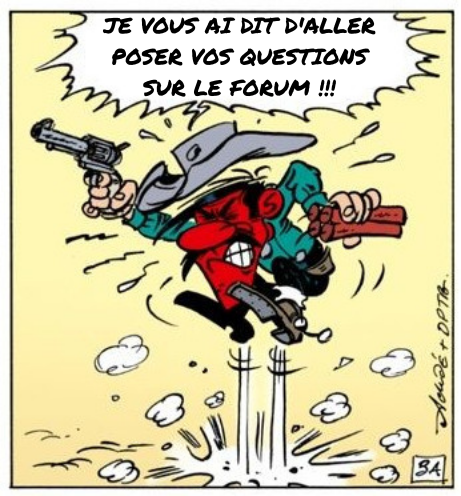
\includegraphics[width=0.7\linewidth]{../../../img/go_forum}
\end{center}
\label{go_forum}
\caption{J'pète les plombs}
\end{figure}}

\newcommand{\reponse}[4][1]
{\noindent
\parbox{\textwidth}{
\rule{\linewidth}{.5pt}\\
\textbf{Question\ifthenelse{#1>1}{s}{} \multido{}{#1}{%
\refstepcounter{num_rep}\ref{q\the\value{num_rep}} }:} ~\ \\
\ifdef{\public}{#3 \ifthenelse{#2>0}{~\ \\ 	\feuilleDR{#2}}}{#4}
}}

\newcommand{\cor}
{\refstepcounter{num_cor}
\noindent
\rule{\linewidth}{.5pt}
\textbf{Question \arabic{num_cor}:} \\
}

\newcommand{\finsujet}
{
    \begin{center}
    \Large{FIN}
    \end{center}

    \cleardoublepage

    \ifdef{\public}{\pagestyle{docreponse}}{\pagestyle{correction}}

    \ifdef{\public}{
        \begin{tikzpicture} 
            \draw (0,0) rectangle (2,2);
            \draw (0,0) -- (2,2);
            \draw (1.5,0.5) node {\large 20};
            \draw (2.5,0) rectangle (16,2);
            \draw (4.5,1.7) node {\large Commentaires:};
        \end{tikzpicture}
    }
    ~\ \\
}


%\newcommand{\repcarre}[2]
%{
%~\ \\
%\begin{tikzpicture}
%\draw [fill=white] (0,0) rectangle +(\linewidth,#1);
%\node[align=left] at (1.1,#2-0.3) {\textbf{Question #1:}};
%\end{tikzpicture}
%}

\newcommand{\titre}[1]
{\begin{center}
\cadre{0.8}{\huge #1} 
\end{center}
}


%Définition des torseurs :
\newcommand{\torseur}[2]{\left\{\mathcal{#1}_{#2} \right\}}
\newcommand{\torseurh}[3]{\left\{\genfrac{}{}{0pt}{0}{#1}{#2}\right\}_{#3}}
\newcommand{\torseurv}[8]{\left\{
\begin{matrix}
#1 & #4 \\ #2 & #5 \\ #3 &#6
\end{matrix}
\right\}_{{#7},{#8}}}

%Définition des torseurs :
%\newcommand{\torseur}[2]{\left \{\mbox{\relsize{2}{$\mathcal {#1}$}\relsize{-2}}\phantom{}_{\mbox{\scriptsize $#2$}} \right \}}
%\newcommand{\torseurh}[3]{\left\{\genfrac{}{}{0pt}{0}{#1}{#2}\right\}_{#3}}
%\newcommand{\torseurv}[8]{
%\left\{\begin{array}{@{}c|c@{}} #1 & #4 \\ #2 & #5 \\ #3 & #6 \end{array} \right\}_{#7,#8}
%}
\newcommand{\derivee}[2]{\left.\dfrac{\d #1}{\d t}\right|_{#2}}
\newcommand{\tripleint}{\int\!\!\!\!\!\int\!\!\!\!\!\int}

% Notation cinématique et statique
\newcommand{\cinematique}[2]{\mbox{#1}/\mbox{#2}}
\newcommand{\statique}[2]{\mbox{#1}\rightarrow\mbox{#2}}
\newcommand{\moment}[3]{\vv {#1}_{\scriptsize{#3}}(#2)}
\newcommand{\resultante}[2]{\vv {#1}_{\scriptsize{#2}}}


%Commande de base
\newcommand{\jo}{\left(j\omega\right)} % j \omega dans l'analyse fréquentielle
\newcommand{\tl}{\xrightarrow{\mathcal{L}}} % transformée de laplace sur fleche
\newcommand{\tli}{\xrightarrow{\mathcal{L}^{-1}}} % transformée inverse de laplace sur fleche
\renewcommand{\d}[1][]{\mathrm{d#1}}
\newcommand{\dd}[1][]{\mathrm{d#1}}
\newcommand{\vect}[2]{{#1}\wedge{#2}}
\newcommand{\base}[3]{(\vec #1,\vec #2,\vec #3)}
\newcommand{\vectbase}[4]{{\vphantom{\left| \begin{matrix}
#1\\#2\\#3 \end{matrix} \right|}}_{#4}{\left| \begin{matrix}
#1\\#2\\#3 \end{matrix} \right.}}
%Pour avoir les paragraphes sous la forme I, II, III
\renewcommand{\thesection}{\Roman{section}}
\setcounter{secnumdepth}{3}
\renewcommand{\Frlabelitemii}{$\bullet$}

% En tête et pied de page
\lhead{\nom}
\rhead{
\includegraphics[width=2cm]{../../../img/logo}}
\lfoot{\auteurun,\ \auteurdeux}
\cfoot{Page \thepage}

\fancypagestyle{docreponse}{%
  \fancyhf{}
  \fancyhead[LO]{NOM Prénom: .............................}
  \rhead{
\includegraphics[width=2cm]{../../../img/logo}\hspace{2pt}}
  \ifdef{\auteurdeux}{\lfoot{\auteurun,\ \auteurdeux}}{\lfoot{\auteurun}}
  \rfoot{\nom}
  \lfoot{Document réponse}
  \cfoot{Page \thepage}
   }

\fancypagestyle{correction}{%
  \fancyhf{}
  \lhead{\colorbox{danger}{\begin{minipage}{0.65\paperwidth} \textcolor{white}{\textbf{Correction}} \end{minipage}} }
  \rhead{
\includegraphics[width=2cm]{../../../img/logo}}
  \lfoot{Renaud Costadoat, Françoise Puig}
  \rfoot{\colorbox{danger}{\begin{minipage}{0.4\paperwidth} \begin{flushright}\textcolor{white}{\textbf{Correction}}\end{flushright} \end{minipage}} }}

\fancypagestyle{correctioninfo}{%
  \fancyhf{}
  \lhead{\colorbox{danger}{\begin{minipage}{0.65\paperwidth} \textcolor{white}{\textbf{Correction}} \end{minipage}} }
  \rhead{
\includegraphics[width=2cm]{../../../img/logo}}
  \lfoot{Renaud Costadoat, Juliette Genzmer}
  \rfoot{\colorbox{danger}{\begin{minipage}{0.6\paperwidth} \begin{flushright}\textcolor{white}{\textbf{Correction}}\end{flushright} \end{minipage}} }}

\renewcommand{\footrulewidth}{0.4pt}

\usepackage{eso-pic}
\newcommand{\BackgroundPic}{%
\put(0,0){%
\parbox[b][\paperheight]{\paperwidth}{%
\vfill
\begin{center}
\hspace{0.5cm}\vspace{0.5cm}

\includegraphics[width=\paperwidth,height=\paperheight,%
keepaspectratio]{../../../img/fond3}%
\end{center}
\vfill
}}}

\newcommand{\BackgroundPicdeux}{%
\put(25,-30){%
\parbox[b][\paperheight]{\paperwidth}{%
\vfill
\begin{center}
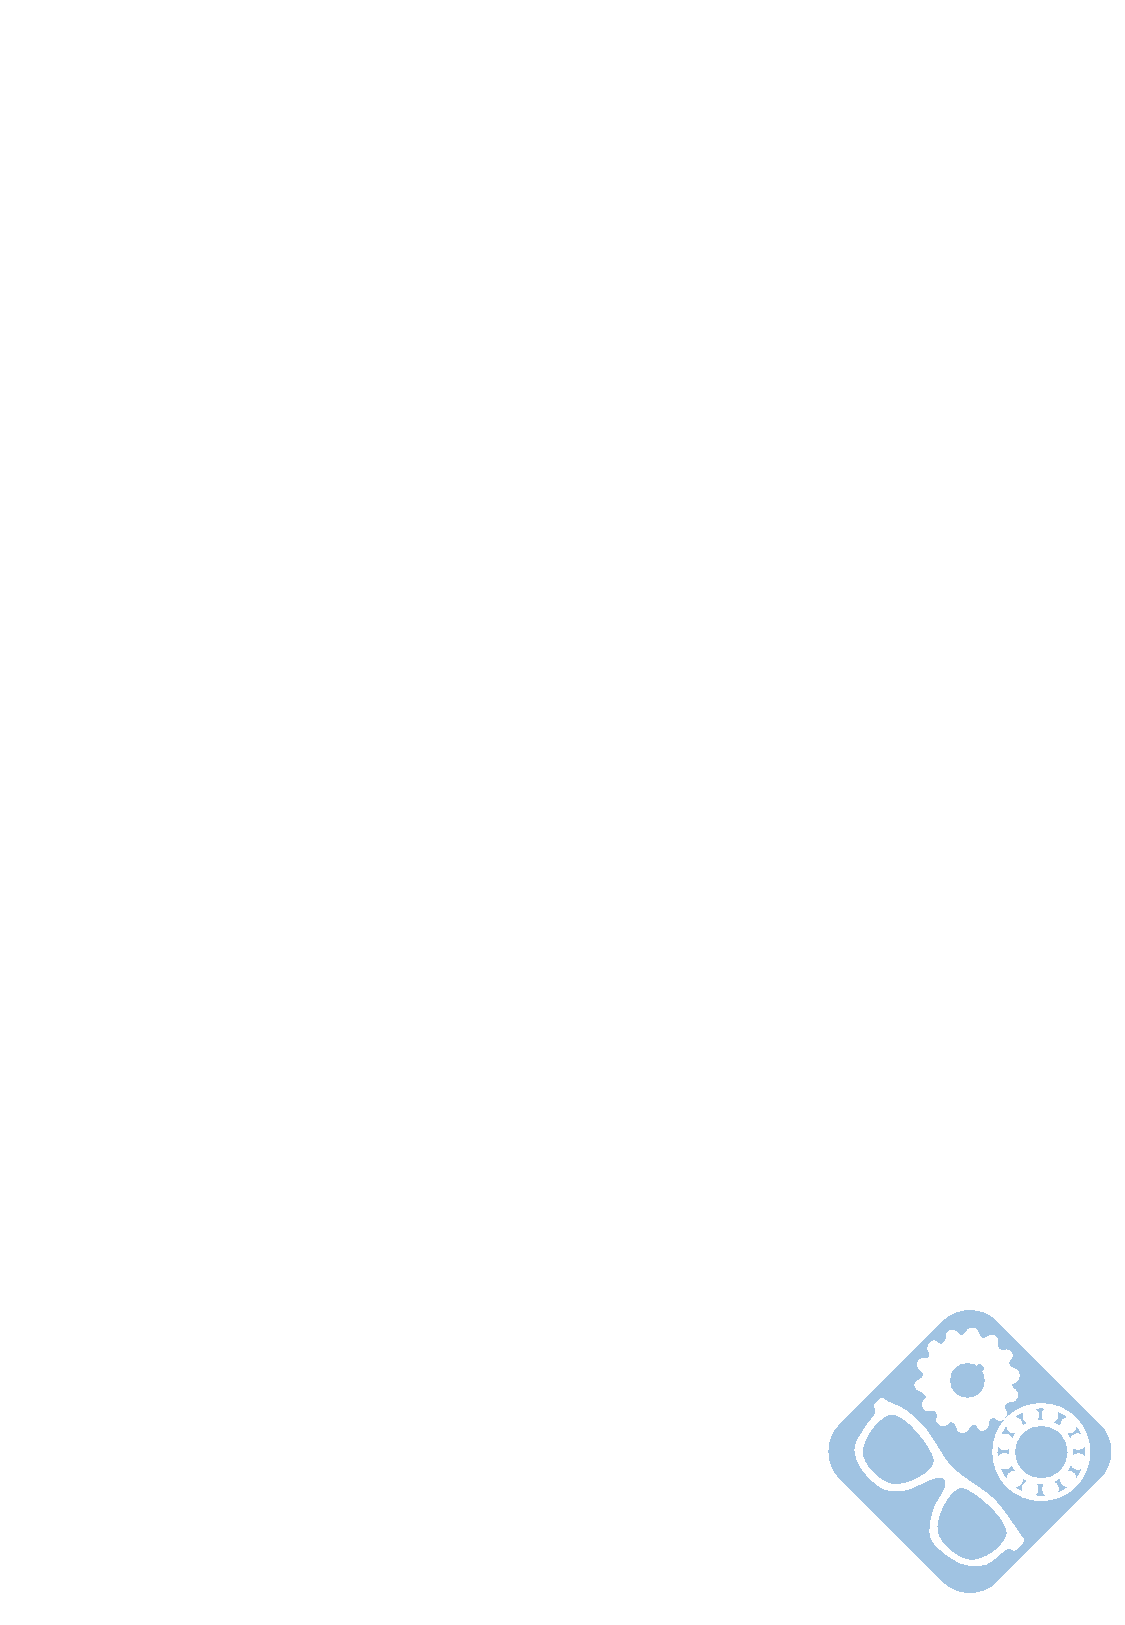
\includegraphics[width=\paperwidth,height=\paperheight,%
keepaspectratio]{../../../img/fond4}%
\end{center}
\vfill
}}}

\begin{document}

\pagestyle{empty}

\AddToShipoutPicture*{\BackgroundPic}


\includegraphics[width=2cm]{../../../img/logo}

\Huge{DS \numero - \sujet}

\vspace{1cm}

\ifdef{\prive}{\begin{center}\colorbox{danger}{\Huge{Avec Correction}}\end{center}}{}

\begin{center}
\centering\huge{PTSI}
\end{center}

\vspace{2cm}


\begin{center}
\centering\Large{\jour}
\end{center}

\vspace{2cm}

\normalsize

\tableofcontents

\newpage

\AddToShipoutPicture{\BackgroundPicdeux}

\pagestyle{fancy}

\begin{center}
\Huge \sujet
\end{center}


\normalsize


\textbf{Notations et informations à respecter:}

\begin{itemize}
 \item Pour écrire un torseur cinématique d'un mouvement de $i/j$, au point $P$, dans le repère $R_0$, vous devrez utiliser uniquement la notation imposée suivante: 

$\left\{V_{i/j}\right\}=\left\{
\begin{matrix}
 \omega x_{ij} & Vx_{P,ij} \\
 \omega y_{ij} & Vy_{P,ij} \\
 \omega z_{ij} & Vz_{P,ij} 
\end{matrix}
\right \}_{P,R_0}=\left \{
\begin{matrix}
 \overrightarrow{\Omega_{i/j}} \\ 
 \overrightarrow{V_{P,i/j}} 
\end{matrix}
\right\}_P$
(l'écriture peut être en ligne ou en colonne)

 \item Pour écrire un torseur d'action mécanique transmissible par une liaison de $i\rightarrow j$, au point $P$, dans le repère $R_0$, vous devrez utiliser uniquement la notation imposée suivante: 

$\left\{T_{i\rightarrow j}\right\}=\left\{
\begin{matrix}
 X_{ij} & {L }_{P,ij} \\
 Y_{ij} & {M }_{P,ij} \\
 Z_{ij} & {N }_{P,ij} 
\end{matrix}
\right \}_{P,R_0}=\left \{
\begin{matrix}
 \overrightarrow{R_{i\rightarrow j}} \\ 
 \overrightarrow{M_{P,i\rightarrow j}} 
\end{matrix}
\right\}_P$
(l'écriture peut être en ligne ou en colonne)

 \item Tous vos résultats seront justifiés.
 \item Vous devrez écrire au stylo, pas au critérium, sinon votre copie ne sera pas corrigée.
 \item Une attention particulière sera apportée au soin de votre copie.
\end{itemize}

\newpage

\section{Système de correction de portée d'un phare automobile}

\subsection{Présentation du système}

L'assiette d'un véhicule se modifie avec sa charge, le profil de la route ou les conditions de conduite (phase de freinage ou d'accélération). Cette modification entraîne une variation d'inclinaison de l'axe du faisceau lumineux produit par les phares du véhicule. Ceux ci peuvent alors éblouir d'autres conducteurs ou mal éclairer la chaussée. 

\begin{figure}[!h]
  \centering
  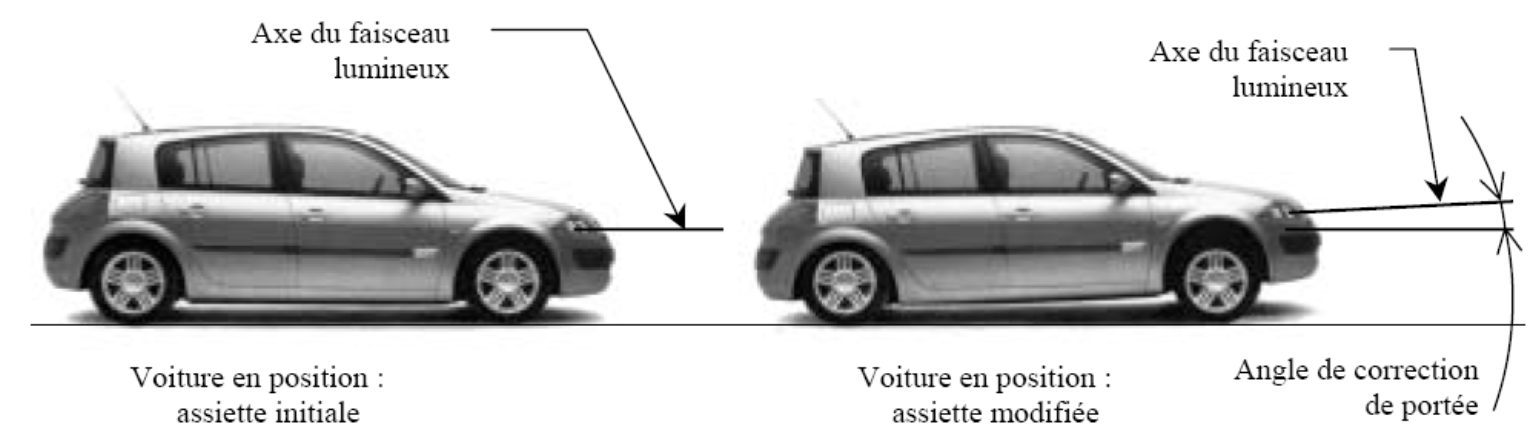
\includegraphics[width=0.9\linewidth]{img/phare1}
  \caption{Correction du faisceau lumineux}
  \label{phare1}
\end{figure}

Certaines voitures sont équipées de système de correction de portée. Ce système fait appel à des capteurs d'assiette reliés aux essieux avant et arrière du véhicule. Les données sont traitées électroniquement par un calculateur et transmises aux actionneurs situés derrière les projecteurs. La position du projecteur est ajustée en maintenant un angle de faisceau optimal évitant tout éblouissement et fournissant le meilleur éclairage de la route.

~\

Le système étudié est un correcteur de portée statique, qui corrige la portée lorsque le véhicule est à l'arrêt et conserve cette correction lorsque le véhicule roule (le correcteur ne tient compte que de la variation d'assiette due à la charge). 

Le but de l'étude est d'analyser le système et de montrer s'il est capable de corriger la portée de manière dynamique, c'est à dire en tenant compte des variations d'assiette dues au profil de la route.

~\

Éléments constitutifs du correcteur de portée :
\begin{itemize}
 \item Capteurs d'assiette : codeurs optiques permettant de mesurer le débattement des suspensions,
 \item Système d'orientation : bloc d'orientation + moto-réducteur + système vis écrou : le bloc d'orientation supporte les différentes lampes du phare (codes, clignotants...). Il peut pivoter par rapport au support lié à la carrosserie autour d'un axe horizontal (axe de rotation indiqué sur la figure ci-dessous). Le bloc est protégé par une vitre liée à la carrosserie. Ce mouvement est motorisé grâce au moto-réducteur + système vis écrou. Il existe aussi une possibilité de réglage manuel en sortie d'usine ou en cas de défaillance du système électrique,
 \item Calculateur : à partir des données des capteurs d'assiette, le calculateur pilote le moto-réducteur.
\end{itemize}

\newpage

\begin{figure}[!h]
  \centering
  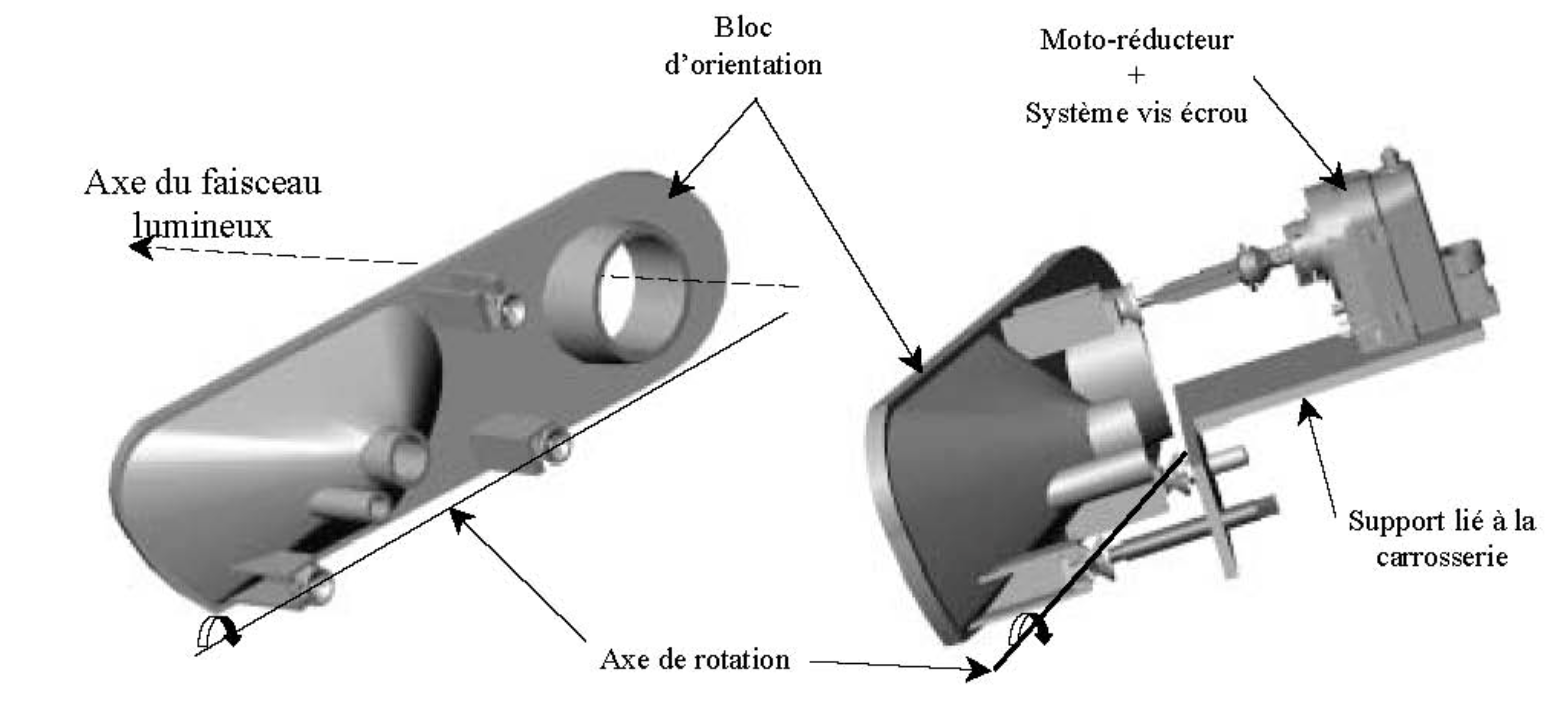
\includegraphics[width=0.8\linewidth]{img/phare2}
  \caption{Système de correction}
  \label{phare2}
\end{figure}

La chaîne d'action complète comprend :

\begin{itemize}
 \item L'ensemble transducteur (capteur + amplificateur + calculateur) qui mesure l'angle de tangage $\beta(t)$ du véhicule et commande le moteur du système. L'ensemble est assimilable à un gain pur $K_C$,
 \item Le moteur à courant continu est alimenté par une tension électrique $U_c(t)$.
$\omega_m(t)$ est la vitesse de l'arbre de sortie du moteur,
 \item On équipe ce moteur d'un retour tachymétrique assimilable à un gain pur $K_{tachy}=0,03 V.rad^{-1}.s$,
 \item Le réducteur de vitesse dont le rapport de réduction est $r=490$. $\omega_r(t)$ est la vitesse de l'arbre de sortie du réducteur, $\theta_r(t)$ est la position angulaire de l'arbre de sortie du réducteur,
 \item L'ensemble vis-écrou (de pas $p_{vis}=6mm$) qui transforme la rotation de l'axe de réducteur en translation de l'axe de sortie (déplacement $x(t)$), (NB : 1 tour de vis fait avancer de 1 pas l'écrou),
 \item Le bloc d'orientation : l'angle de correction de portée $\theta(t)$ étant petit, on peut linéariser la loi entrée-sortie sur le domaine d'utilisation : l'angle $\theta(t)$ est proportionnel au déplacement $x(t)$ de la vis. $\theta(t)$ varie entre $-\frac{\pi}{20}$ et $\frac{\pi}{20}$ pour $x(t)$ compris entre $-15mm$ et $+15mm$.
\end{itemize}

\subsection{Etude fonctionnelle}

\paragraph{Question 1:} Compléter sur le document réponse:
\begin{itemize}
 \item le schéma fonctionnel en indiquant les unités en entrée et sortie de chaque bloc fonctionnel,
 \item le tableau en indiquant la fonction de chaque bloc fonctionnel.
\end{itemize}

\subsection{Transformées de Laplace: Schéma bloc du système}

Les notations pour les transformées de Laplace des différentes variables temporelles sont les suivantes :
\begin{math}
\begin{array}{c c c}
L[\beta(t)]=B(p) &  L[\omega_m(t)]=\Omega_m(p) &  L[U_c(t)]=U_c(p) \\
L[\theta_r(t)]=\Theta_r(p) &  L[\omega_r(t)]=\Omega_r(p) &  L[x(t)]=X(p) \\
\end{array}
\end{math}

La fonction de transfert du moteur seul sera notée $M(p)$.

\paragraph{Question 2:} En citant les théorèmes utilisés, trouver une relation entre $\Omega_r(p)$ et $\Theta_r(p)$.

\paragraph{Question 3:} Écrire la relation qui lie $x(t)$ et $\theta_r(t)$ (donc entre le déplacement de la vis et la position angulaire de la vis) et en citant les théorèmes utilisés, trouver une relation entre $X(p)$ et $\Theta_r(p)$.

\paragraph{Question 4:} Compléter le schéma bloc sur le document réponse en remplissant chaque bloc par la fonction de transfert correspondante.

\subsection{Etude du moteur}

Dans cette partie, vous allez trouver l'expression littérale et numérique de la fonction de transfert $M'(p)=\frac{\Omega_m(p)}{U_c(p)}$ (moteur et retour tachymétrique), à l'aide de la réponse temporelle du moteur (seul) à une sollicitation en échelon.

La réponse indicielle est donnée sur la figure \ref{phare3}:

\begin{figure}[!h]
  \centering
  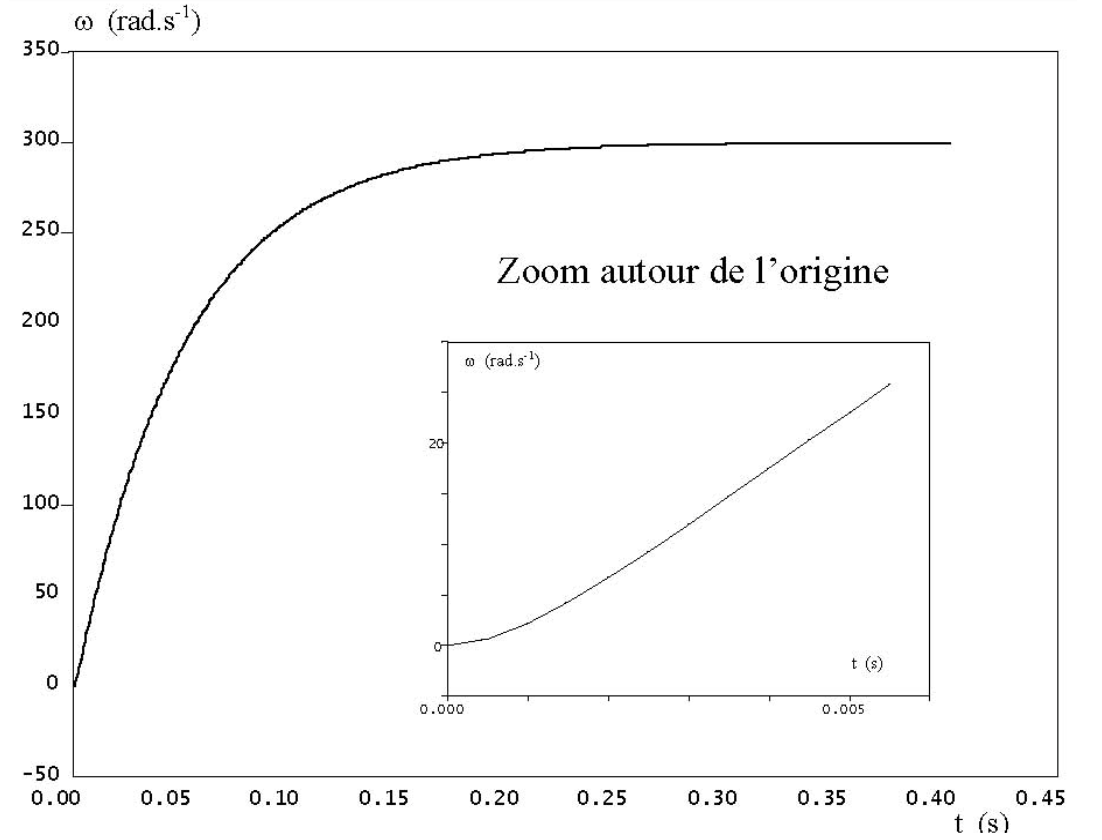
\includegraphics[width=0.6\linewidth]{img/phare3}
  \caption{Réponse indicielle}
  \label{phare3}
\end{figure}

\paragraph{Question 5:} D'après la figure \ref{phare3}, quelle est la valeur de la tangente à l'origine de cette courbe ?

\paragraph{Question 6:} D'après la figure \ref{phare3}, quelle est la valeur de l'asymptote de cette courbe en $+\infty$ ?

\paragraph{Question 7:} Déduire de vos réponses aux questions 5 et 6 la forme de la fonction de transfert $M(p)$ du moteur.

\paragraph{Question 8:} Quelle hypothèse fait-on pour assimiler la fonction de transfert de ce moteur à un premier ordre ?

\paragraph{Question 9:} Ecrire la nouvelle fonction de transfert $M(p)$ sous forme canonique (en faisant l'hypothèse d'un système du premier ordre) et trouvez les valeurs numériques des paramètres caractéristiques de ce premier ordre. Vous indiquerez les unités.

\paragraph{Question 10:} Après avoir rappelé la définition du temps de réponse à 5\% d'un système asservi, trouver la valeur numérique de ce temps de réponse pour le moteur étudié à l'aide de la figure \ref{phare3}.

\paragraph{Question 11:} Démontrer que l'hypothèse faite à la question 8 est vérifiée.

\paragraph{Question 12:} Trouver la fonction de transfert prenant en compte le retour tachymétrique $M'(p)=\frac{\Omega_m(p)}{U_c p)}$.

\subsection{Chaîne d'action complète}

Le véhicule est brusquement chargé à l'arrière (assimilable à un échelon).

Quelles que soient les réponses précédentes, on donne la fonction de transfert de la chaîne d'action complète:

\begin{center}
$H(p)=\frac{\Theta(p)}{B(p)}=K_C.\frac{0,003}{p.(1+0,025.p)}$
\end{center}

Les angles d'entrée et de sortie sont exprimés en radians.

\paragraph{Question 13:} Tracer SANS CALCUL l'allure de l'entrée et l'allure de la réponse à un échelon pour ce système.

\paragraph{Question 14:} Donner la définition de l'écart statique $\epsilon_S$ et calculer sa valeur pour le système étudié (citer le/les théorème(s) utilisé(s)). Conclure quant à la précision du système. 

\subsection{Retour tachymétrique}

Pour pallier ce problème, on asservit en position le système en plaçant :
\begin{itemize}
 \item Un capteur de position, de gain $K_{pos}$,
 \item Un amplificateur $A$.
\end{itemize}

\begin{figure}[!h]
  \centering
  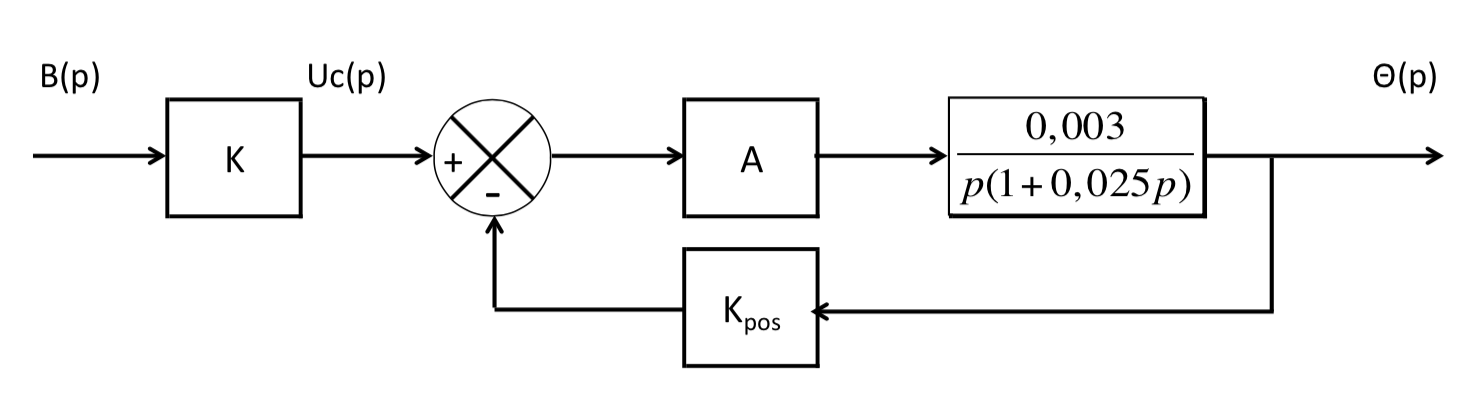
\includegraphics[width=0.6\linewidth]{img/phare4}
  \caption{Boucle de retour tachymétrique}
  \label{phare4}
\end{figure}

\paragraph{Question 15:} Déterminez la fonction de transfert et toutes les caractéristiques de $H'(p)=\frac{\Theta(p)}{B(p)}$.

\paragraph{Question 16:} Quelle est la nouvelle valeur de l'écart statique ? 

\paragraph{Question 17:} Quelle(s) modification(s) le retour tachymétrique a-t-il donc apporté ?

\paragraph{Question 18:} Quelle doit être la valeur de $A.K_{pos}$ pour avoir le temps de réponse le plus petit ?

\paragraph{Question 19:} Donner alors cette valeur de $t_{r5\%}$. (Vous utiliserez la courbe figure \ref{phare5} donnant le temps de réponse réduit $t_{r5\%}.\omega_n$ en fonction du coefficient d'amortissement $z$).

\paragraph{Question 20:} Quelle est alors la valeur du premier dépassement ? (Vous utiliserez la courbe \ref{phare5} donnant les dépassements successifs en fonction du coefficient d'amortissement $z$).

\paragraph{Question 21:} Quelle doit être la valeur de $A.K_{pos}$ pour avoir le temps de réponse le plus petit, sans dépassement ?

\begin{figure}[!h]
  \centering
  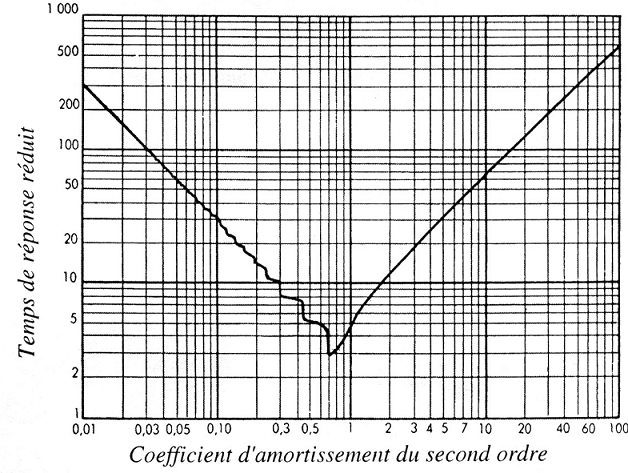
\includegraphics[width=0.6\linewidth]{img/phare5}
  \caption{$t_{r5\%}.\omega_n$=fonction(z)}
  \label{phare5}
\end{figure}

\begin{figure}[!h]
  \centering
  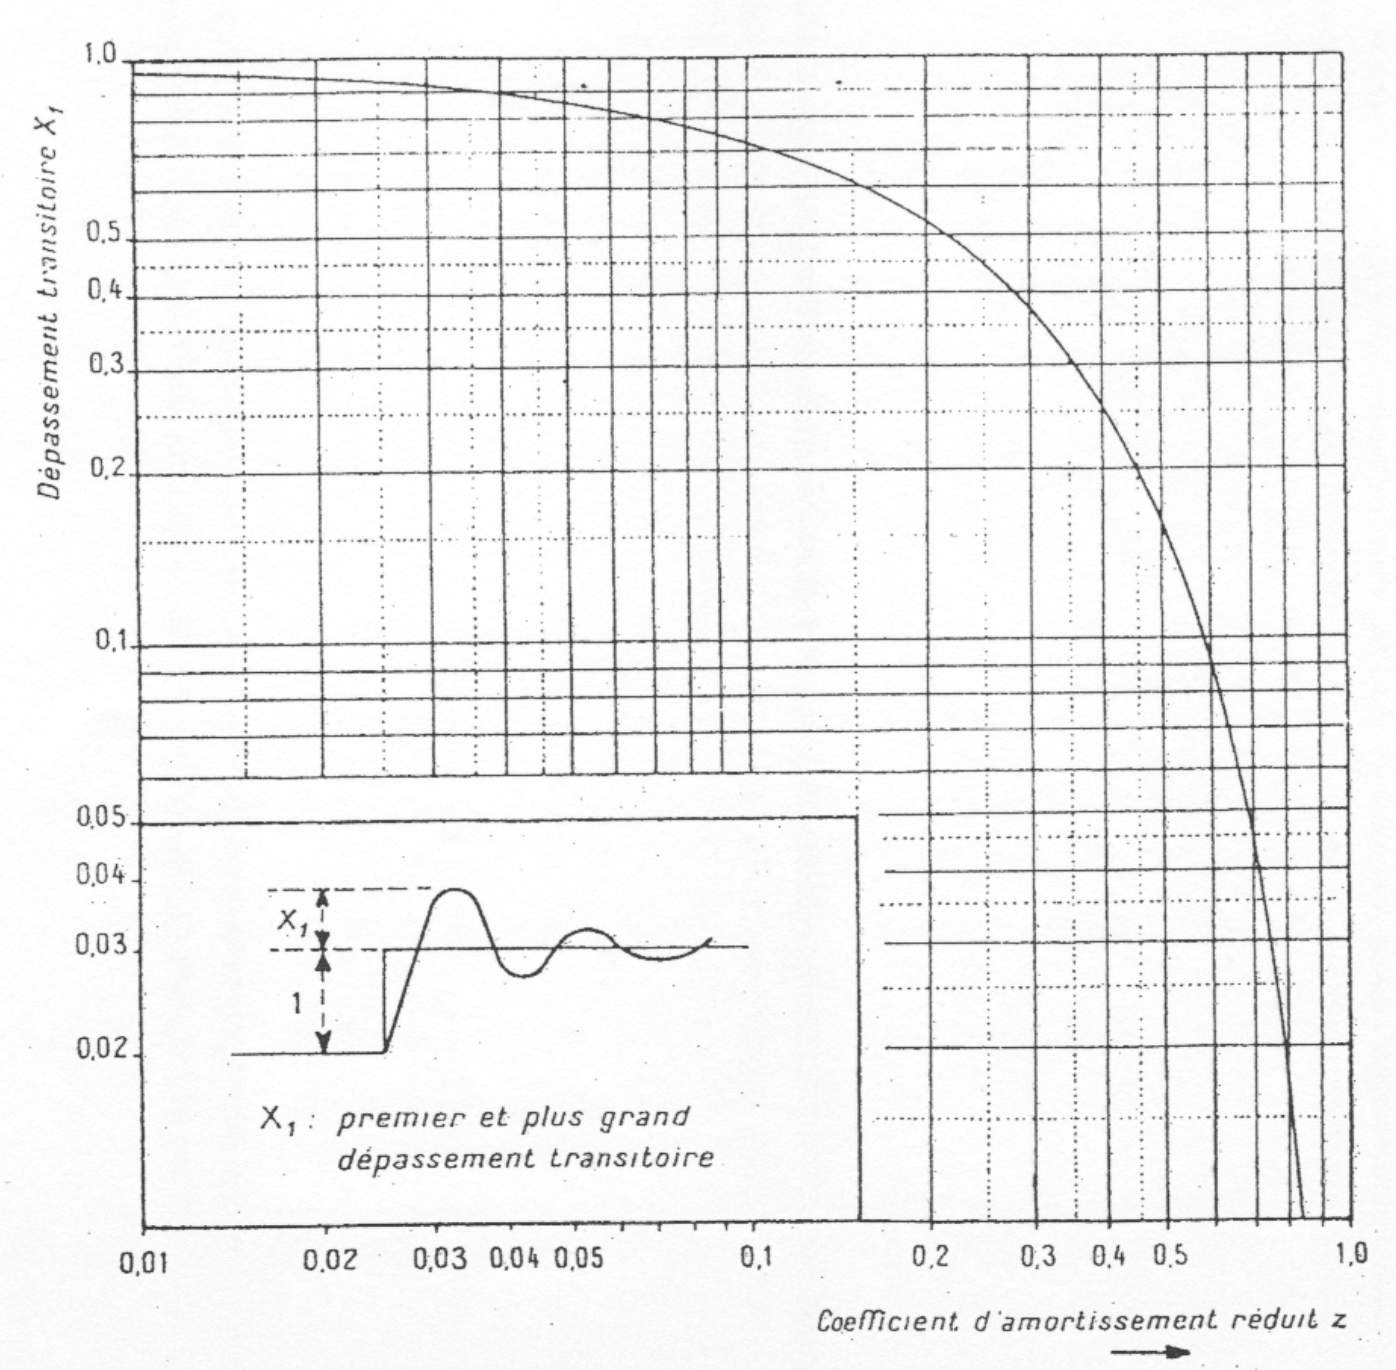
\includegraphics[width=0.6\linewidth]{img/phare6}
  \caption{(dépassement X\textsubscript{1}) = fonction (z)}  
  \label{phare6}
\end{figure}

\subsection{Etude de l'orientation de l'axe optique}

\subsubsection{Etude de la chaîne cinématique : motoréducteur + système vis écrou}

La chaîne cinématique est constituée d'un moteur électrique 208, de 2 réducteurs roue et vis sans fin (209 / 210a et 210b / 203) et d'un double système vis écrou (réglage manuel et réglage motorisé).

\begin{figure}[!h]
  \centering
  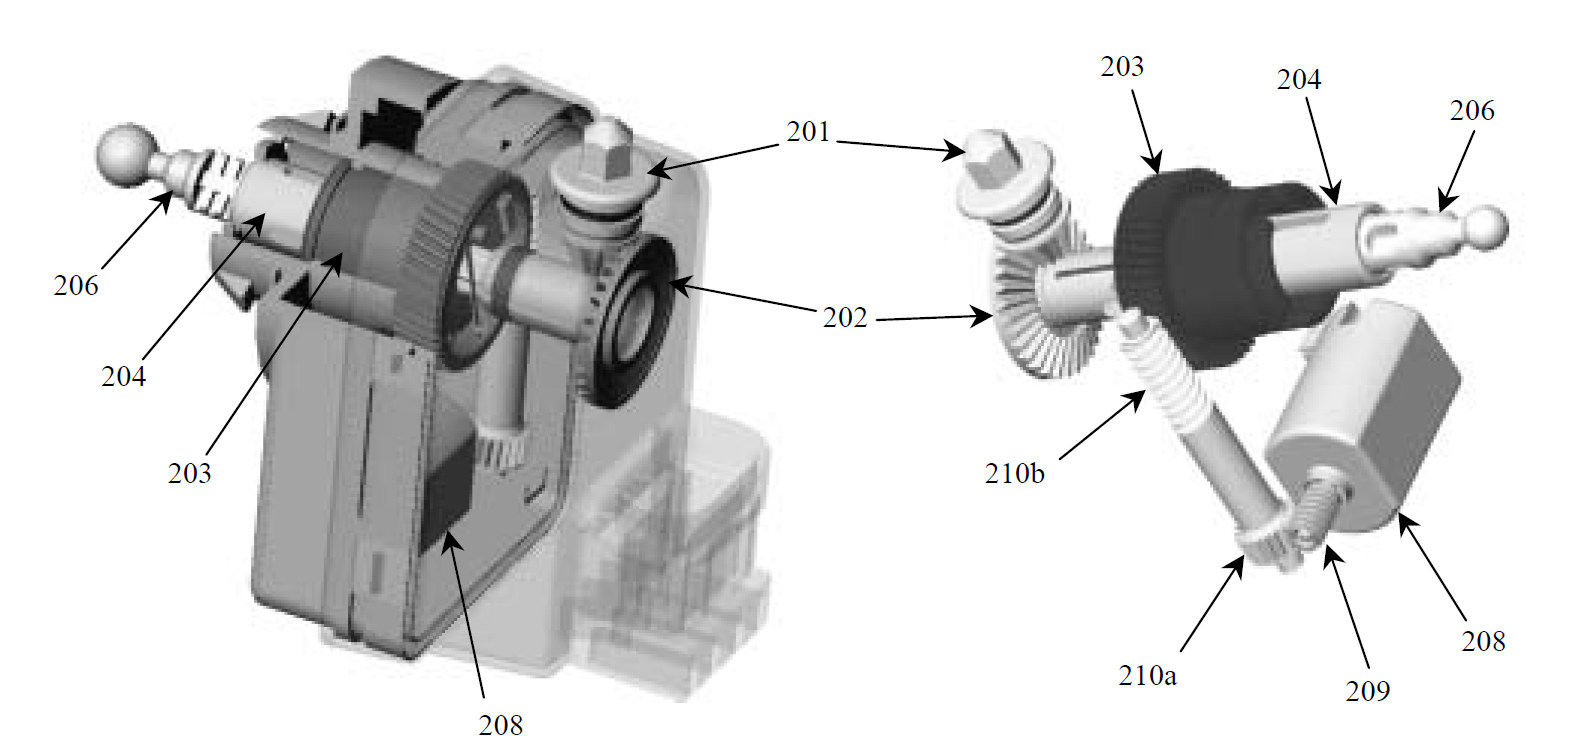
\includegraphics[width=0.8\linewidth]{img/phare7}
  \caption{Vue avec boîtier gauche (un quart enlevé) et boîtier droit translucide/Vue sans boîtier}  
  \label{phare7}
\end{figure}

Le moteur 208 entraîne en rotation la vis sans fin 209 qui entraîne la roue 210a par un système roue et vis sans fin. La vis 210b entraîne à son tour la roue 203 par un autre système roue et vis sans fin.

\textbf{Mode motorisé :} Un système vis 204 écrou 203 permet de transformer la rotation de la roue 203 en une translation de la tige 206 (liée à 204 en mode motorisé). Celle-ci permet l'orientation du phare par l'intermédiaire de la biellette de poussée 303 (voir schéma cinématique).

\begin{figure}[!h]
  \centering
  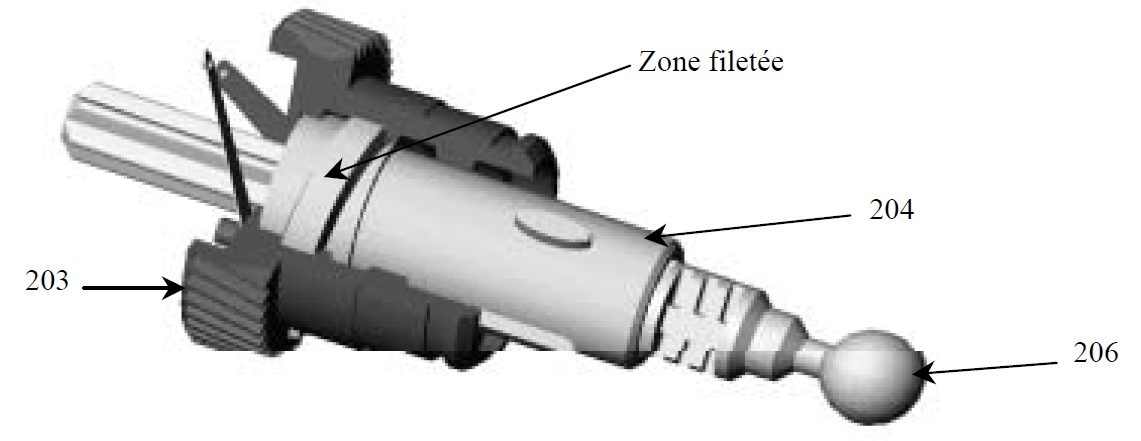
\includegraphics[width=0.6\linewidth]{img/phare8}
  \label{phare8}
\end{figure}

\textbf{Mode manuel :} La rotation du bouton de réglage manuel 201 permet la rotation de la vis 206 par l'intermédiaire de l'engrenage conique 201 - 202 et de cannelures entre 202 et 206. L'écrou 204 étant fixe en mode manuel la vis 206 a donc un mouvement hélicoïdal.

\begin{figure}[!h]
  \centering
  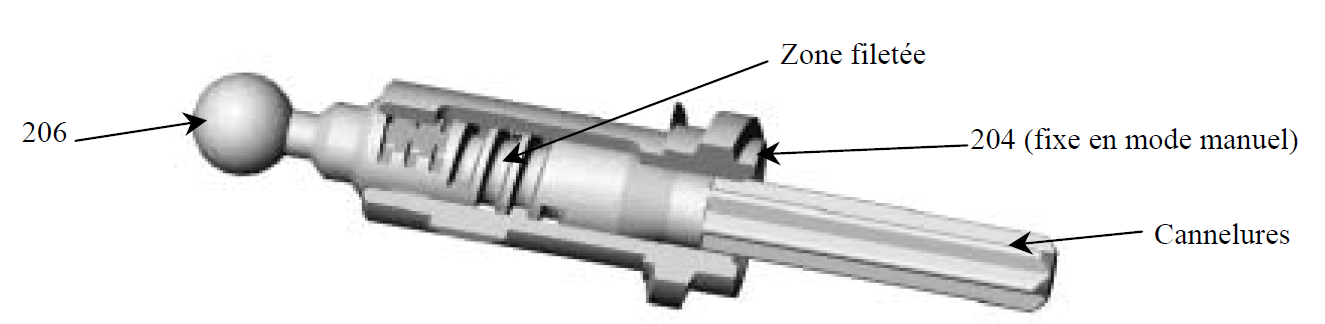
\includegraphics[width=0.6\linewidth]{img/phare9}
  \label{phare9}
\end{figure}

Le système motoréducteur et vis écrou est modélisé par le schéma cinématique suivant :

\begin{figure}[!h]
  \centering
  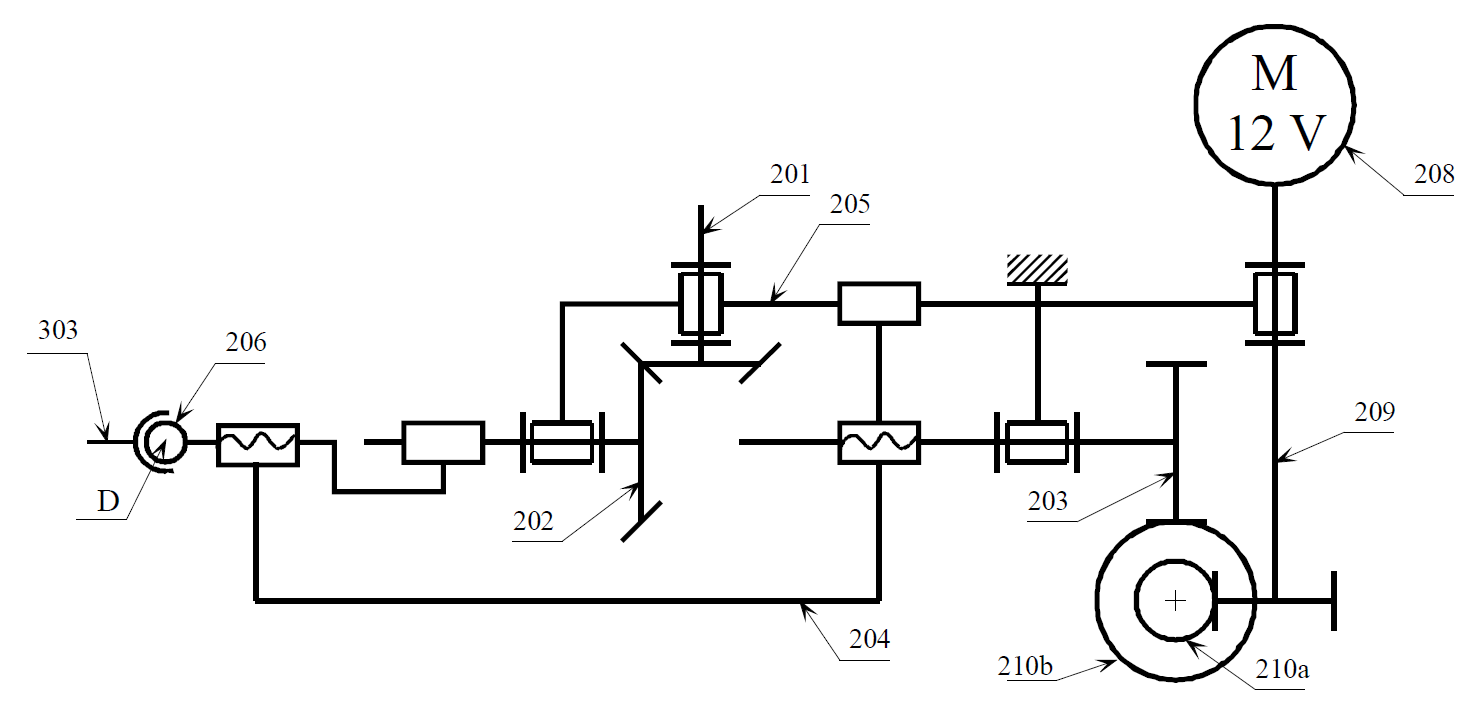
\includegraphics[width=0.6\linewidth]{img/phare10}
  \label{phare10}
\end{figure}

\paragraph{Question 22:} Sur le document réponse, pour le réglage motorisé et le réglage manuel, surligner en vert les pièces ayant un mouvement de rotation par rapport au bâti. Surligner en bleu les pièces ayant un mouvement de translation par rapport au bâti. Surligner en rouge les pièces ayant un mouvement de rotation et translation par rapport au bâti.

\paragraph{Question 23:} Sur le dessin d'ensemble du document réponse, colorier en vert, sur toutes les vues l'écrou 204.

\subsubsection{Etude de l'orientation du bloc optique}

Voir le système d'orientation en annexe.

Deux liaisons en A et B permettent au boîtier 301 de pivoter par rapport au bâti autour d'un axe ($A,\overrightarrow{y}$).

La liaison rotule de centre A est réalisée par une pièce intermédiaire en plastique, 302, clipsée sur un embout sphérique lié au bâti 304 et fixé sur le boîtier 301.

La liaison linéaire annulaire en B est réalisée par une pièce plastique 302 identique clipsée sur un embout sphérique lié au bâti 304 mais en liaison glissière de direction $\overrightarrow{y}$ par rapport au boitier 301.

\begin{figure}[!h]
  \centering
  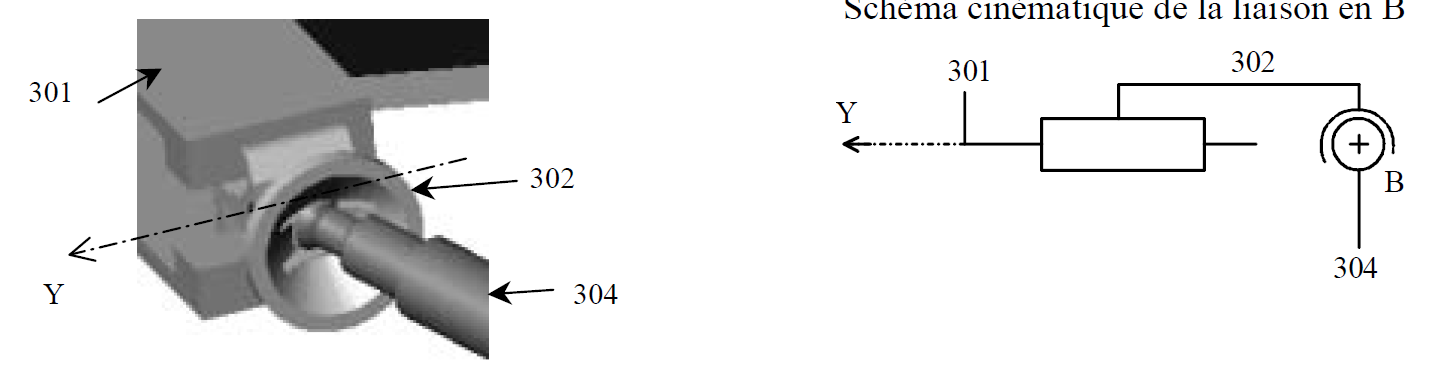
\includegraphics[width=0.6\linewidth]{img/phare11}
  \caption{Liaison en B/Schéma cinématique de la liaison en B}
  \label{phare11}
\end{figure}

\paragraph{Question 24:} Ecrire les torseurs suivants $\left\{V_{304/302}\right\}$ et $\left\{V_{302/301}\right\}$ au point B. En déduire le torseur $\left\{V_{304/301}\right\}$.

Démontrer par les torseurs que la liaison équivalente en B est une liaison linéaire annulaire d'axe ($B,\overrightarrow{y}$).

\paragraph{Question 25:} La liaison en A étant une liaison rotule, et celle en B une linéaire annulaire d'axe ($B,\overrightarrow{y}$), donner sans calcul la liaison équivalente entre le boîtier 301 et le bâti 304 en ne tenant compte que des liaisons en A et B.

\paragraph{Question 26:} Tracer sur le document réponse, dans le cas d'un réglage motorisé, le schéma cinématique minimal dans le plan ($A,\overrightarrow{x},\overrightarrow{z}$) de la chaîne fermée constituée du bâti 304 et des pièces 301, 206 et 303.

La position définie sur l'épure, document réponse 3, correspond à une position extrême 0 (points $A$, $C$ et $D$).

On notera $A$, $C_1$ et $D_1$ les points dans l'autre configuration extrême 1.

\paragraph{Question 27:} En supposant la course de l'axe 206 égale à 30 mm ($\overrightarrow{DD_1}=3°0.\overrightarrow{x}$), tracer sur le document réponse le point $C_1$, les pièces 301 et 303 et l'axe du faisceau lumineux. Mesurer l'amplitude angulaire du faisceau.

\newpage

\section{Robot préhenseur de pièces}

\begin{minipage}{0.45\linewidth}
On s'intéresse à un robot préhenseur de pièces dont on donne une description structurelle ainsi qu'un extrait partiel du diagramme des exigences de son modèle SysML. L'objectif de cette étude est de vérifier les performances d'un des axes asservis de ce robot vis-à-vis des critères de performances attendus. \\
	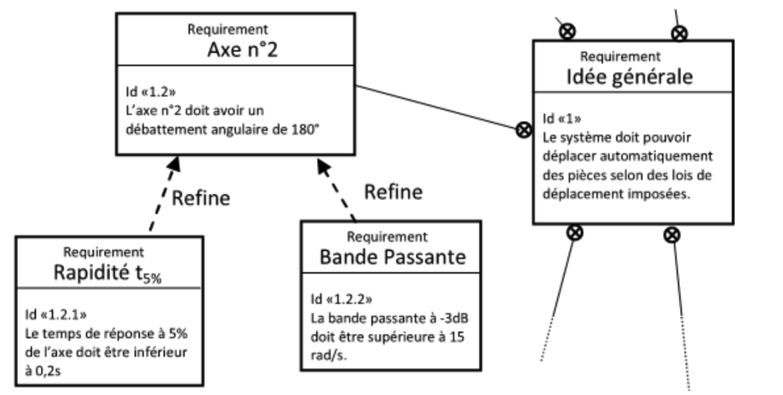
\includegraphics[width=0.8\linewidth]{img/robot1}
\end{minipage}\hfill
\begin{minipage}{0.45\linewidth}
	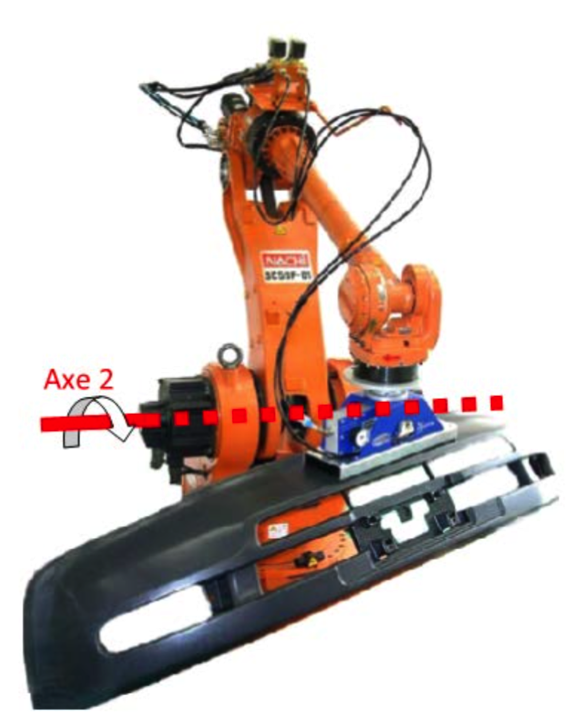
\includegraphics[width=0.9\linewidth]{img/robot2}
\end{minipage}

On donne le modèle de comportement de l'asservissement de position angulaire de l'axe du bras étudié sous la forme du schéma bloc qui suit. L'angle réel du bras est $\theta(t)$, l'angle de consigne est $\theta_c(t)$.

\begin{figure}[!h]
  \centering
  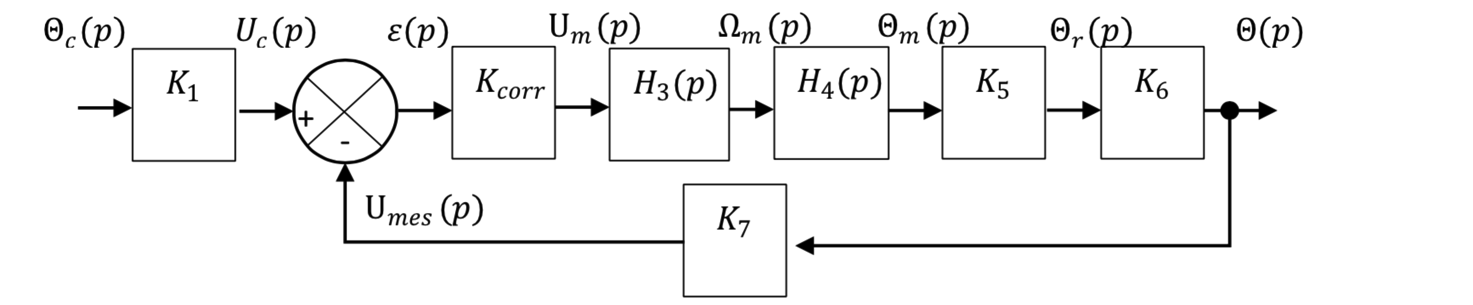
\includegraphics[width=0.6\linewidth]{img/robot3}
  \label{robot3}
\end{figure}

\begin{minipage}{0.45\linewidth}
Avec $K_1$, $K_{corr}$, $K_5$, $K_6$, $K_7$: constantes.
\begin{itemize}
 \item $\Theta_c(p)$: angle de consigne,
 \item $U_c(p)$: angle de consigne,
 \item $U_m(p)$: tension moteur,
 \item $\Omega_m(p)$: vitesse angulaire de l'arbre moteur,
\end{itemize} 
\end{minipage}\hfill
\begin{minipage}{0.45\linewidth}
\begin{itemize}
 \item $\Theta_m(p)$: angle de l'arbre moteur,
 \item $\Theta_r(p)$: angle de l'arbre en sortie de réducteur,
 \item $\Theta(p)$: position angulaire du bras,
 \item $U_{mes}(p)$: tension mesurée image de $\Theta(p)$.
\end{itemize}
\end{minipage}

\paragraph{Question 28:} Déterminer le lien entre $K_1$ et $K_7$ pour que le système soit correctement asservi, donc quand $\epsilon(t)$ tend vers 0.

La fonction de transfert $H_3(p)$ est représentative d'un moteur dont on connaît le modèle de comportement, au travers des équations suivantes :

~\

\begin{minipage}[t]{0.45\linewidth}
$u_m(t)=e(t)+R.i(t)$, $e(t)=k_e.\omega_m(t)$ \\
Avec:
\begin{itemize}
 \item $u_m(t)$: tension aux bornes du moteur(V),
 \item $e(t)$: force contre-électromotrice(V),
 \item $i(t)$: intensité (A),
 \item $\omega_m(t)$: vitesse de rotation de l'arbre en sortie de moteur($rad.s^{-1}$),
 \item $c_m(t)$: couple moteur (N.m),
\end{itemize}
\end{minipage}\hfill
\begin{minipage}[t]{0.45\linewidth}
$J.\frac{d \omega_m(t)}{dt}=c_m(t)$, $c_m(t)=k_m.i(t)$ \\
~\
\begin{itemize}
 \item $J$: inertie équivalente en rotation de l'arbre moteur ($kg.m^2$),
 \item $R$: résistance électrique du moteur ($\Omega$),
 \item $k_e$: constante de force contre-électromotrice ($V.rad^{-1}$),
 \item $k_m$: constante de couple ($N.m.A^{-1}$).
\end{itemize}
\end{minipage}

\paragraph{Question 29:} Déterminer la fonction de transfert $H_3(p)=\frac{\Omega_m(p)}{U_m(p)}$ en citant le/les théorèmes utilisés. Montrer qu'on peut la mettre sous la forme $H_3(p)=\dfrac{K_3}{1+\tau_3.p}$ et donner l'expression littérale de $\tau_3$.

\paragraph{Question 30:} Déterminer $\omega_m(t)$ quand on sollicite le système avec une entrée de type échelon de valeur $u_m(t)=U_0.u(t)$ avec $u(t)$ fonction de Heaviside.

\paragraph{Question 31:} Tracer la courbe sur le document réponse et positionner toutes les caractéristiques propres à un système du premier ordre soumis à un échelon.

\paragraph{Question 32:} Déterminer la fonction de transfert $H_4(p)$ en citant le/les théorèmes utilisés.

\paragraph{Question 33:} Déterminer la fonction de transfert $H(p)=\frac{\theta(p)}{\theta_c(p)}$. Montrer qu'on peut la mettre sous la forme $H(p)=\frac{K_0}{1+\frac{2.z}{\omega_n}.p+\frac{1}{\omega_n^2}.p^2}$ et déterminer les valeurs littérales de $K_0$, $\omega_n$ et $z$ en fonction des constantes fournies.

La réponse indicielle de $H(p)$ est donnée ci-dessous :
\begin{figure}[!h]
  \centering
  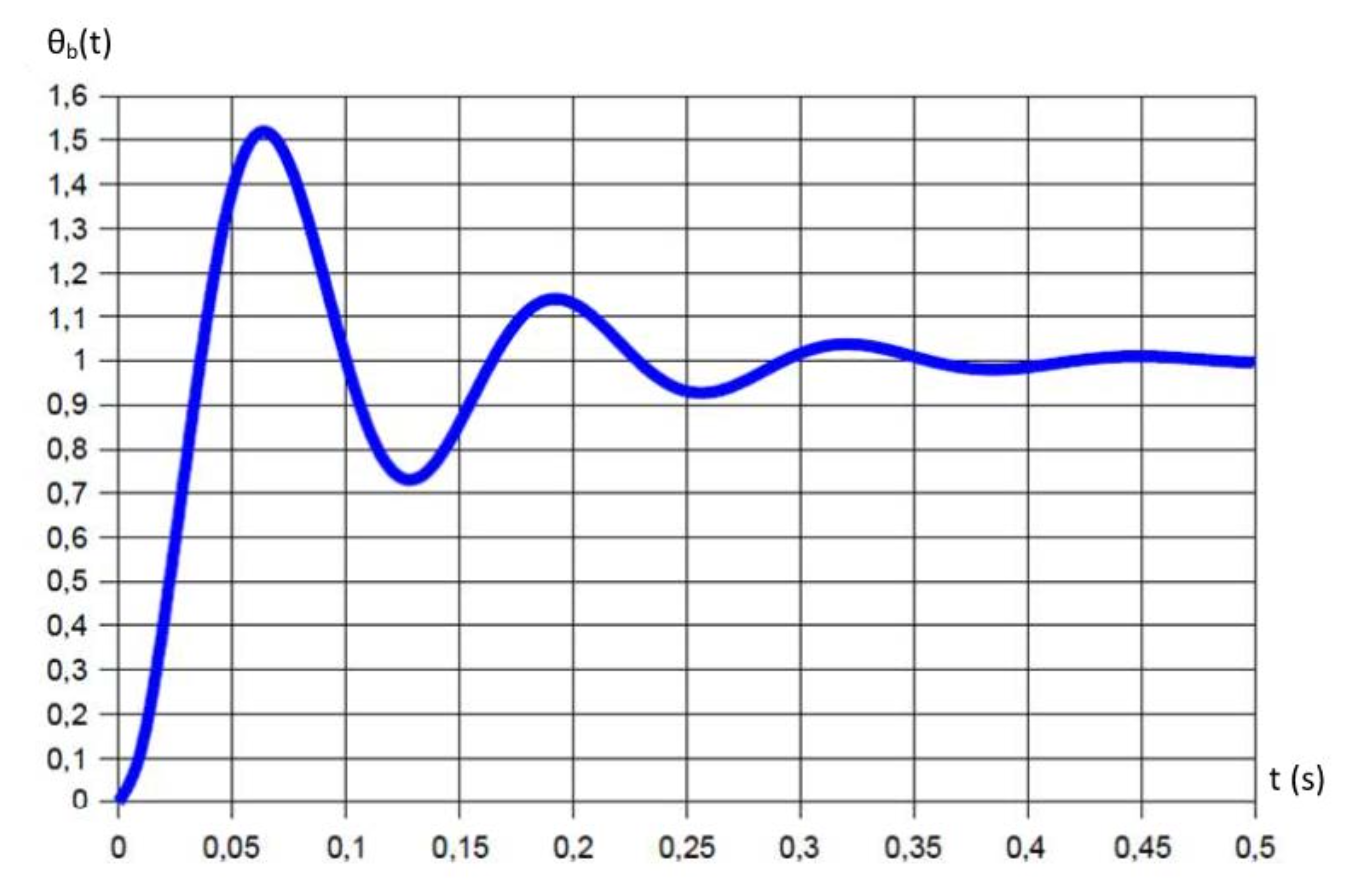
\includegraphics[width=0.6\linewidth]{img/robot4}
  \label{robot4}
\end{figure}

\paragraph{Question 34:} Déterminer les valeurs numériques de $K_0$, $\omega_n$ et $z$, en expliquant votre démarche (voir les figures \ref{phare5} et \ref{phare6}).

\paragraph{Question 35:} Déterminer le temps de réponse à 5\%, en expliquant votre démarche (voir les figures \ref{phare5} et \ref{phare6}).

\paragraph{Question 36:} Conclure quant à la capacité du préhenseur de pièce à vérifier (ou non) le cahier des charges fourni, en terme de rapidité.

\section{Torseur d'action mécanique transmissible par une liaison}

\paragraph{Question 37:} Compléter le tableau sur le document réponse (en respectant les notations) pour les différentes liaisons proposées.

\section{Assemblage vissé dans une lance de distribution}

Le système suivant est une lance de distribution d'essence.

\begin{center}
 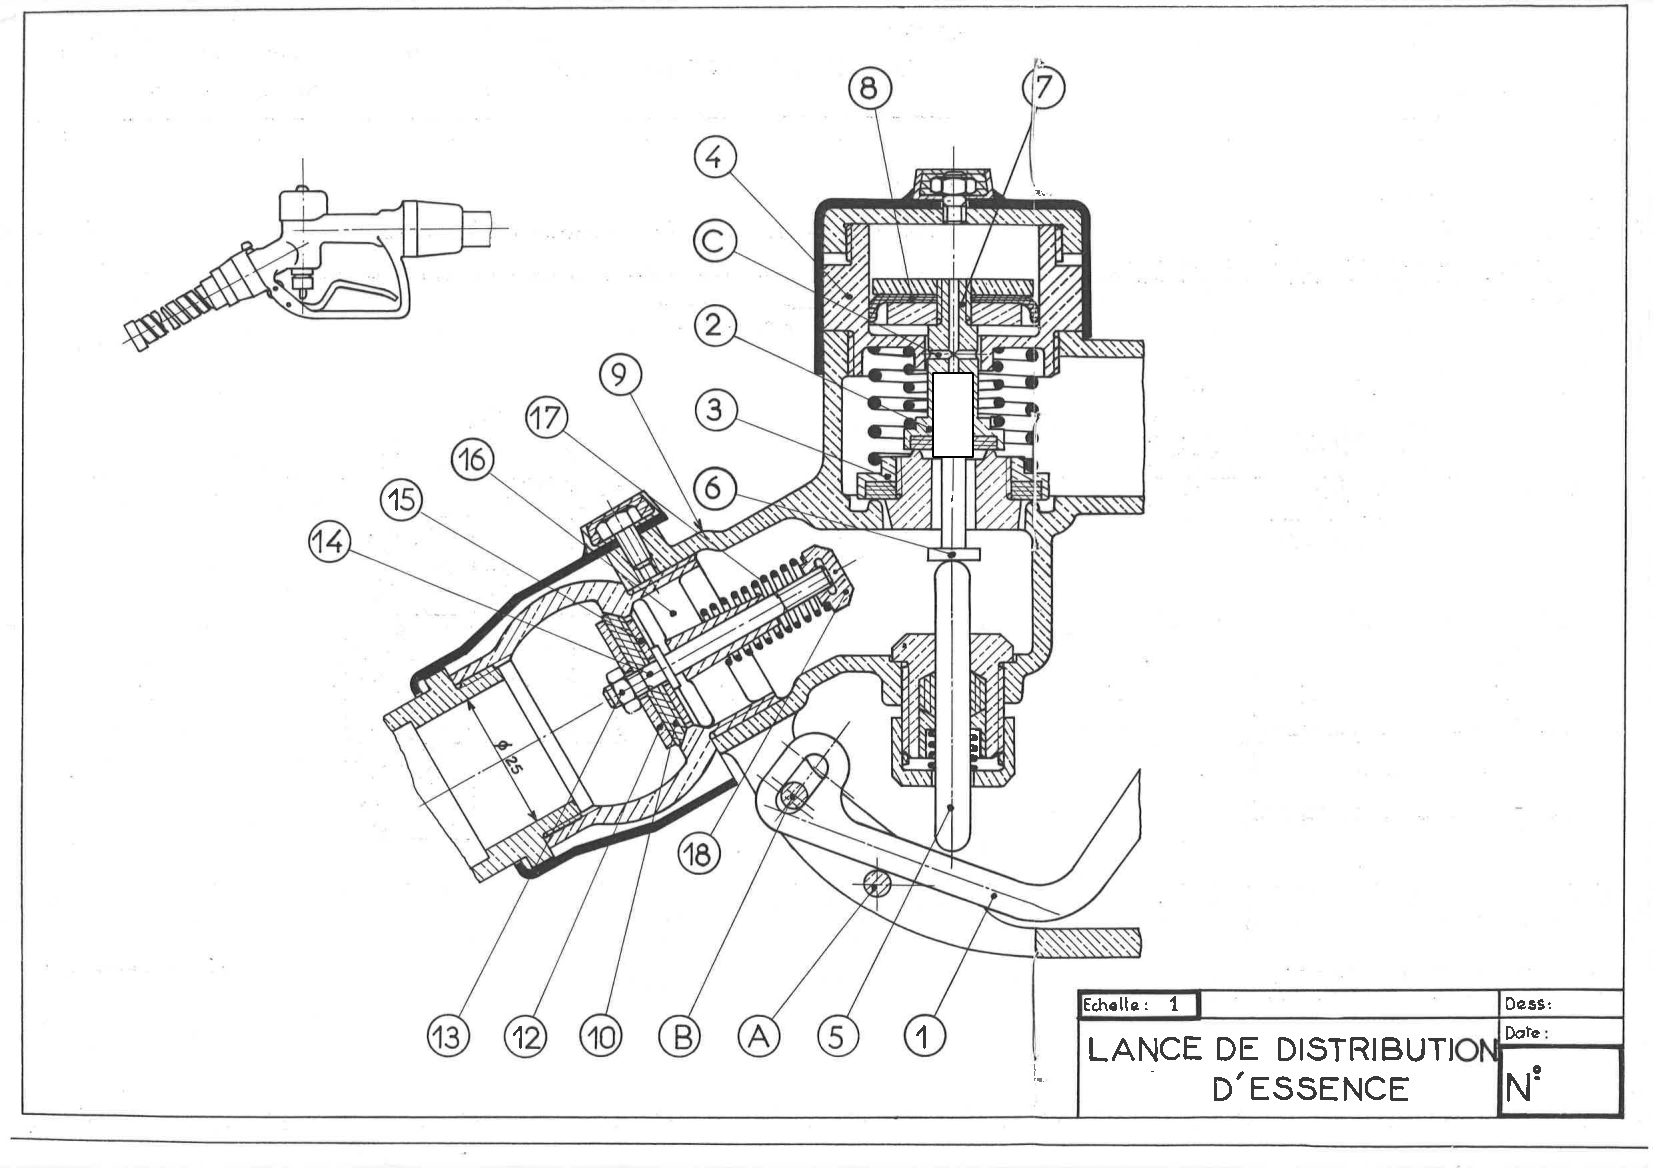
\includegraphics[width=\linewidth]{img/lance}
\end{center}

\begin{minipage}{0.7\linewidth}
La vis 6 permet de transmettre le mouvement de la gâchette 1 à la pièce 7 qui permet de laisser passer ou de bloquer l'essence.

Celle-ci est représenté à droite. Sa mise en place sur le système est à concevoir.

\paragraph{Question 38:} Proposer, sur le document réponse, une solution d'assemblage démontable de la pièce 6 sur la pièce 7. Les tracés ne devront apparaître qu'à l'intérieur du rectangle blanc.
\end{minipage}\hfill
\begin{minipage}{0.25\linewidth}
 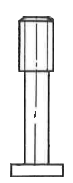
\includegraphics[width=0.5\linewidth]{img/vis}
\end{minipage}

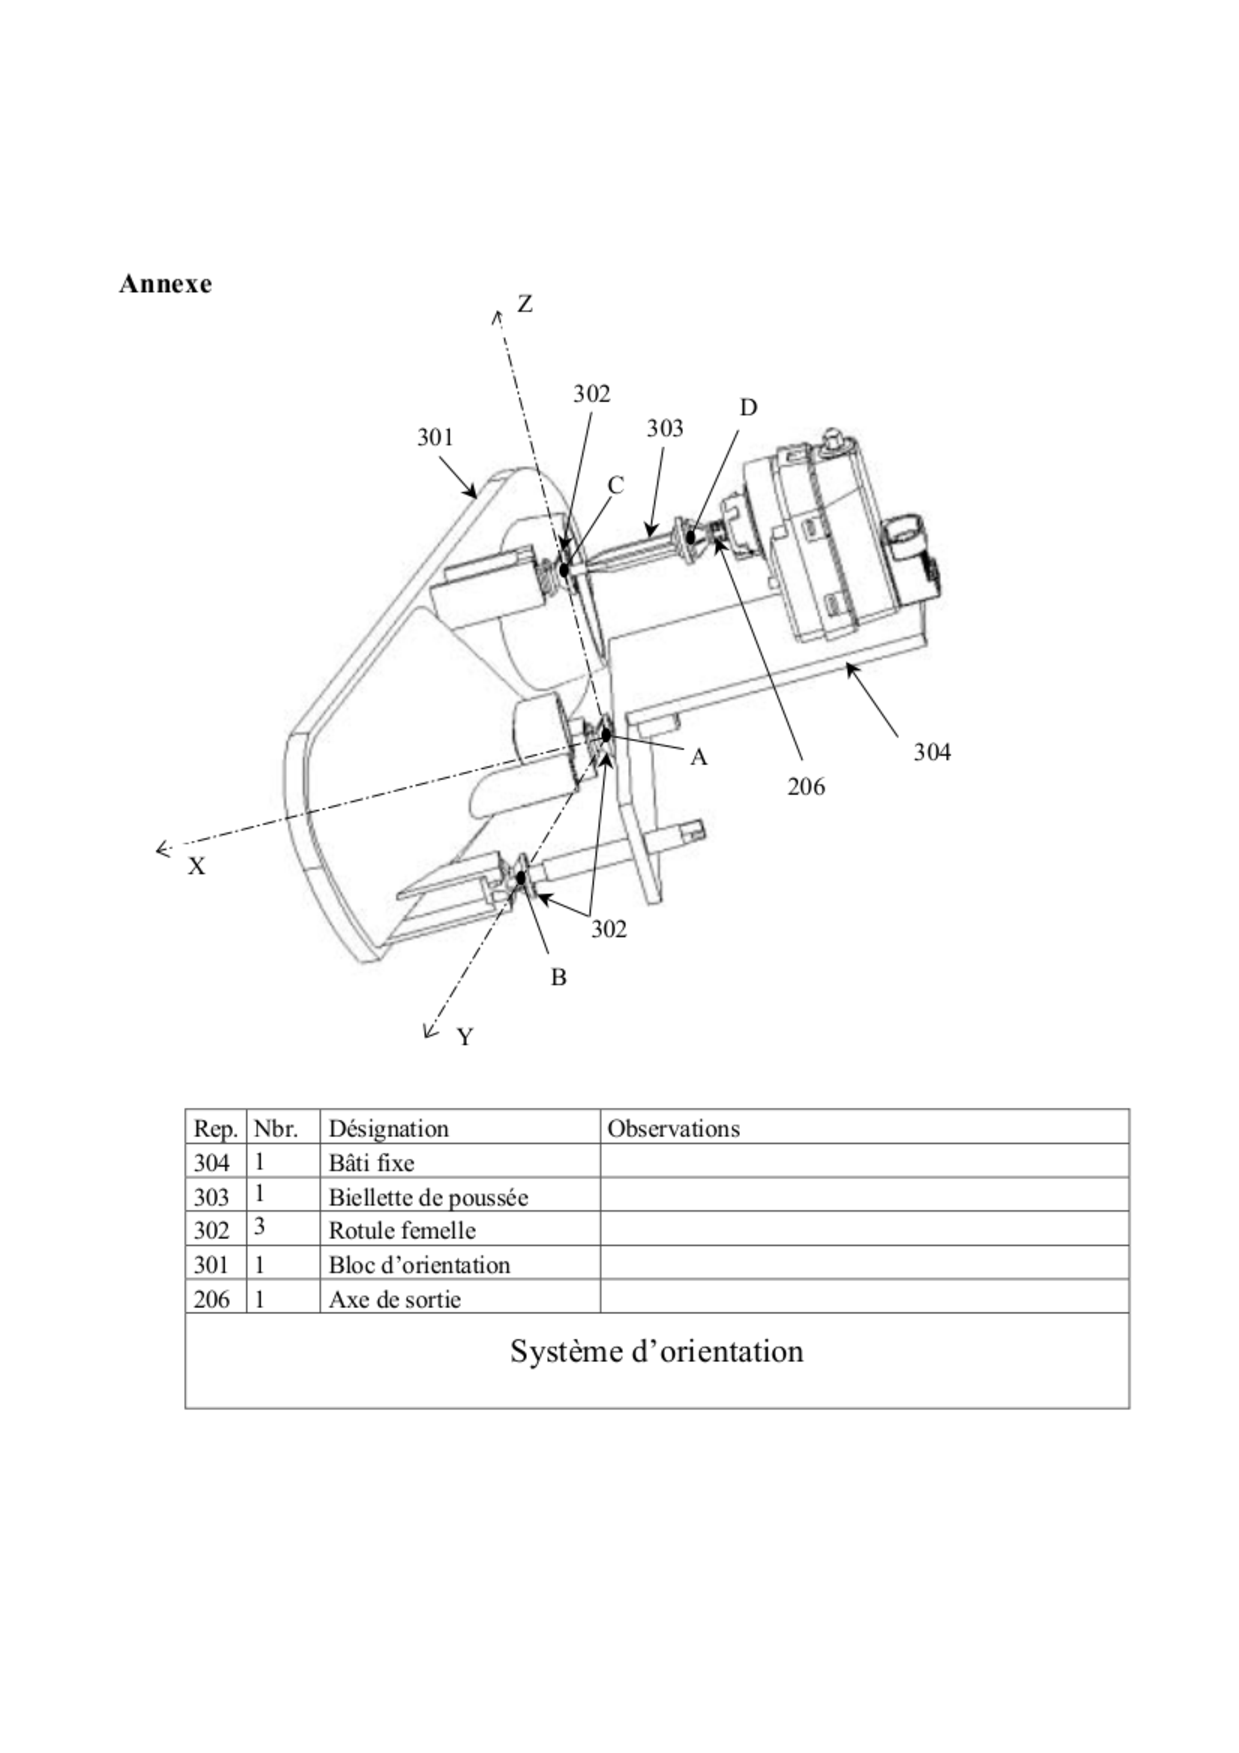
\includepdf[pages=1]{img/annexe.pdf}

\cleardoublepage

\pagestyle{documentreponse}

\section{Document réponse}

\subsection{Correcteur de portée de phare}

\paragraph{Question 1:}

\begin{center}
  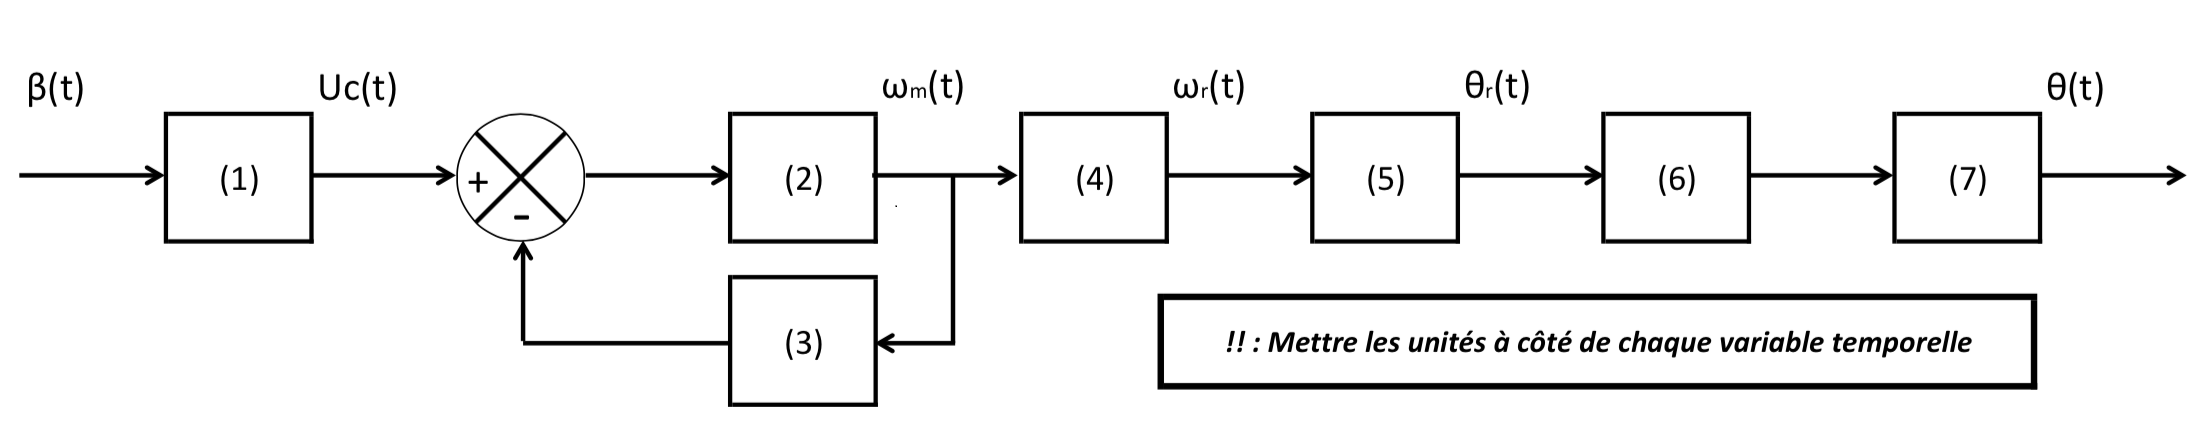
\includegraphics[width=0.8\linewidth]{img/rep1}

\begin{tabular}{|c|m{10cm}|}
\hline
 & Fonction \\
\hline
 (1) & \\
  ~\ & \\
\hline
 (2) & \\
  ~\ & \\
\hline
 (3) & \\
  ~\ & \\
\hline
 (4) & \\
  ~\ & \\
\hline
 (5) & \\
  ~\ & \\
\hline
 (6) & \\
  ~\ & \\
\hline
 (7) & \\
  ~\ & \\
\hline
\end{tabular}
\end{center}

\paragraph{Question 2:}

\reponse[4]


\paragraph{Question 3:}

\reponse[4]

\paragraph{Question 4:}

\begin{center}
  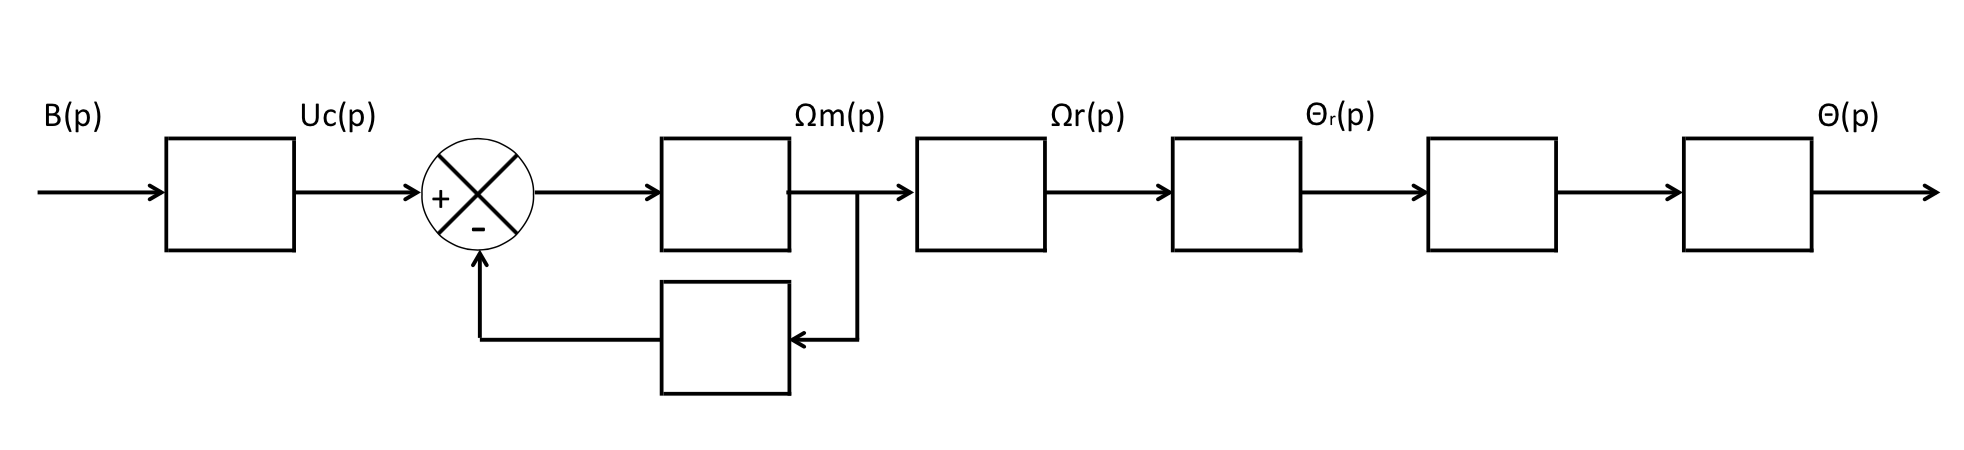
\includegraphics[width=0.9\linewidth]{img/rep2}
\end{center}

\paragraph{Question 5:}

\begin{center}
  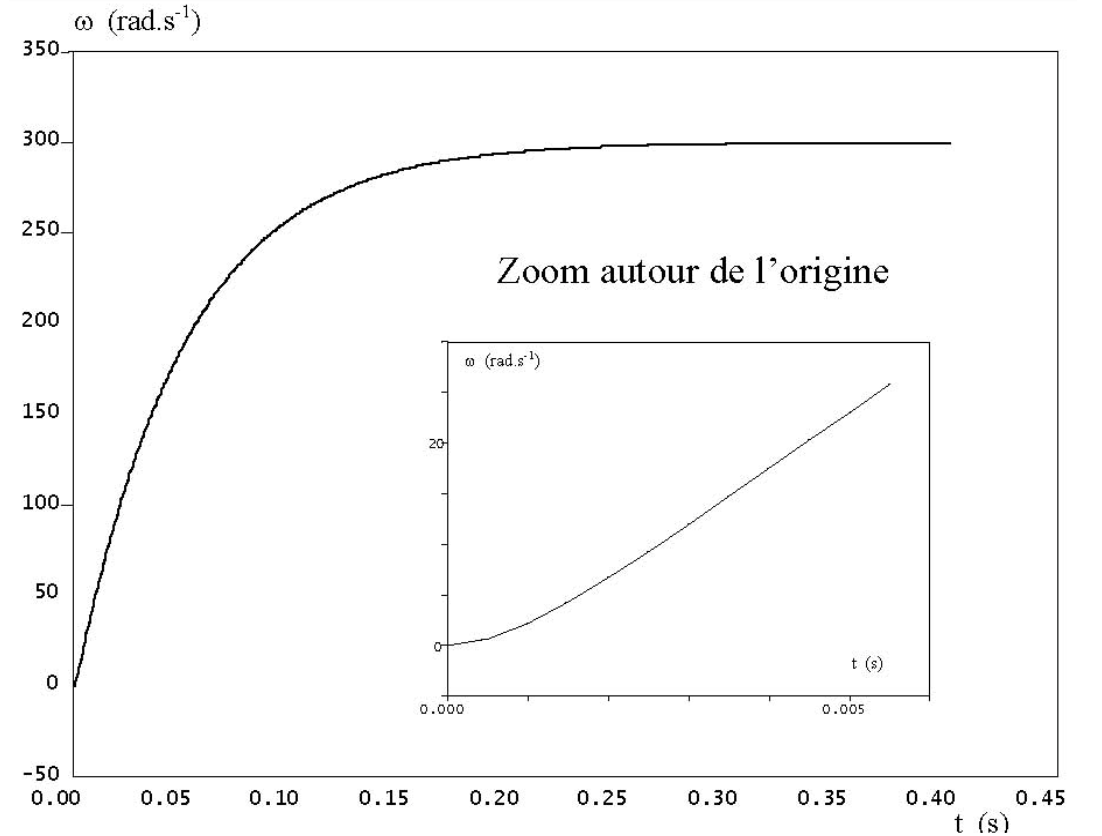
\includegraphics[width=0.6\linewidth]{img/rep3}
\end{center}

\reponse[2]

\paragraph{Question 6:}

\reponse[2]

\paragraph{Question 7:}

\reponse[3]

\paragraph{Question 8:}

\reponse[3]

\paragraph{Question 9:}

\reponse[3]

\paragraph{Question 10:}

\reponse[3]

\paragraph{Question 11:}

\reponse[3]

\paragraph{Question 12:}

\reponse[4]

\paragraph{Question 13:}

\begin{center}
\begin{minipage}{0.49\linewidth}
	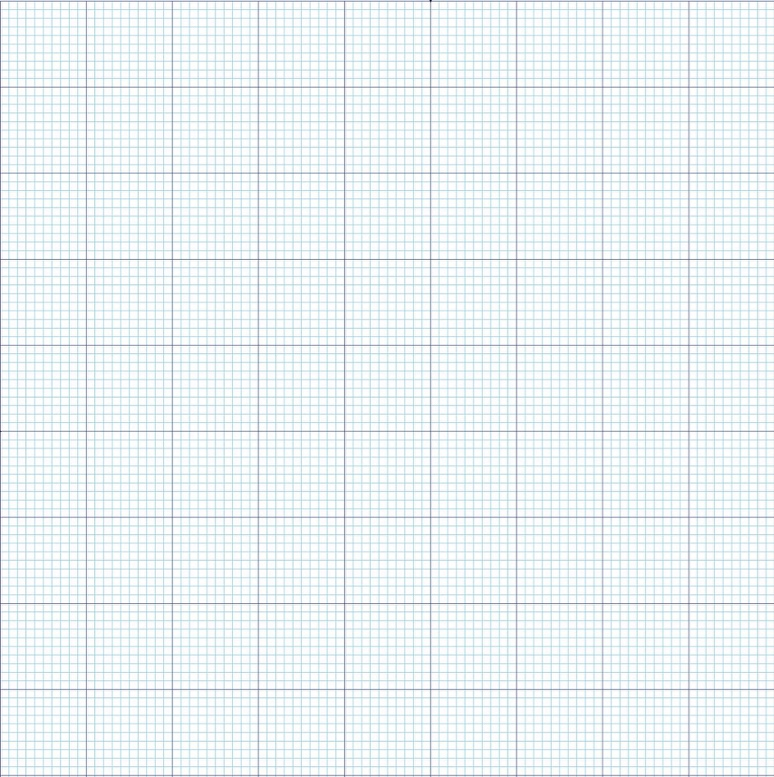
\includegraphics[width=\linewidth]{img/rep4}
\end{minipage}\hfill
\begin{minipage}{0.49\linewidth}
	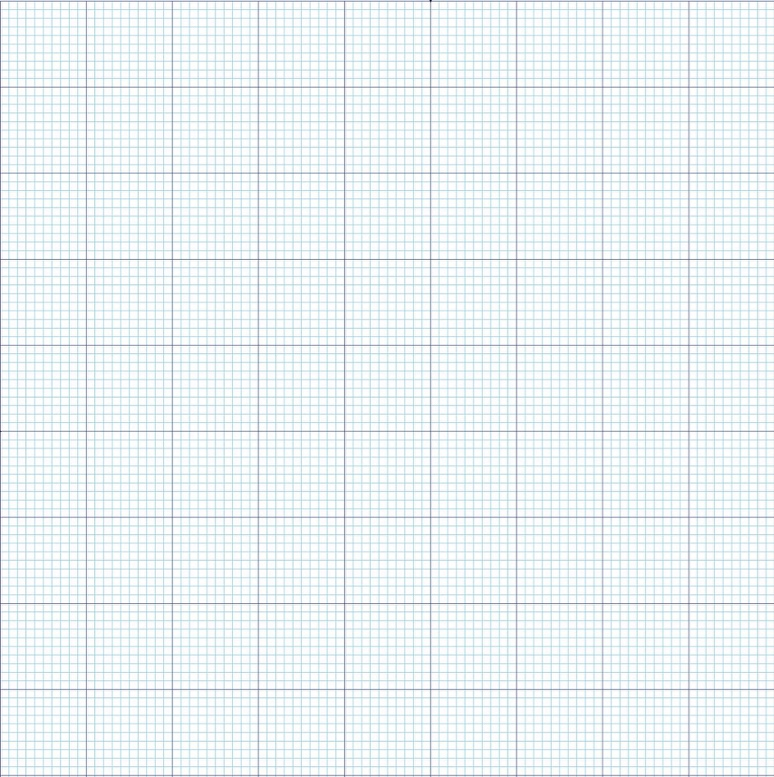
\includegraphics[width=\linewidth]{img/rep4}
\end{minipage}
\end{center}

\paragraph{Question 14:}

\reponse[3]

\paragraph{Question 15:}

\reponse[3]

\paragraph{Question 16:}

\reponse[3]

\paragraph{Question 17:}

\reponse[4]

\paragraph{Question 18:}

\reponse[3]

\paragraph{Question 19:}

\reponse[2]

\paragraph{Question 20:}

\reponse[2]

\paragraph{Question 21:}

\reponse[4]

\newpage

\paragraph{Question 22:}

~\

Réglage motorisé

\begin{center}
  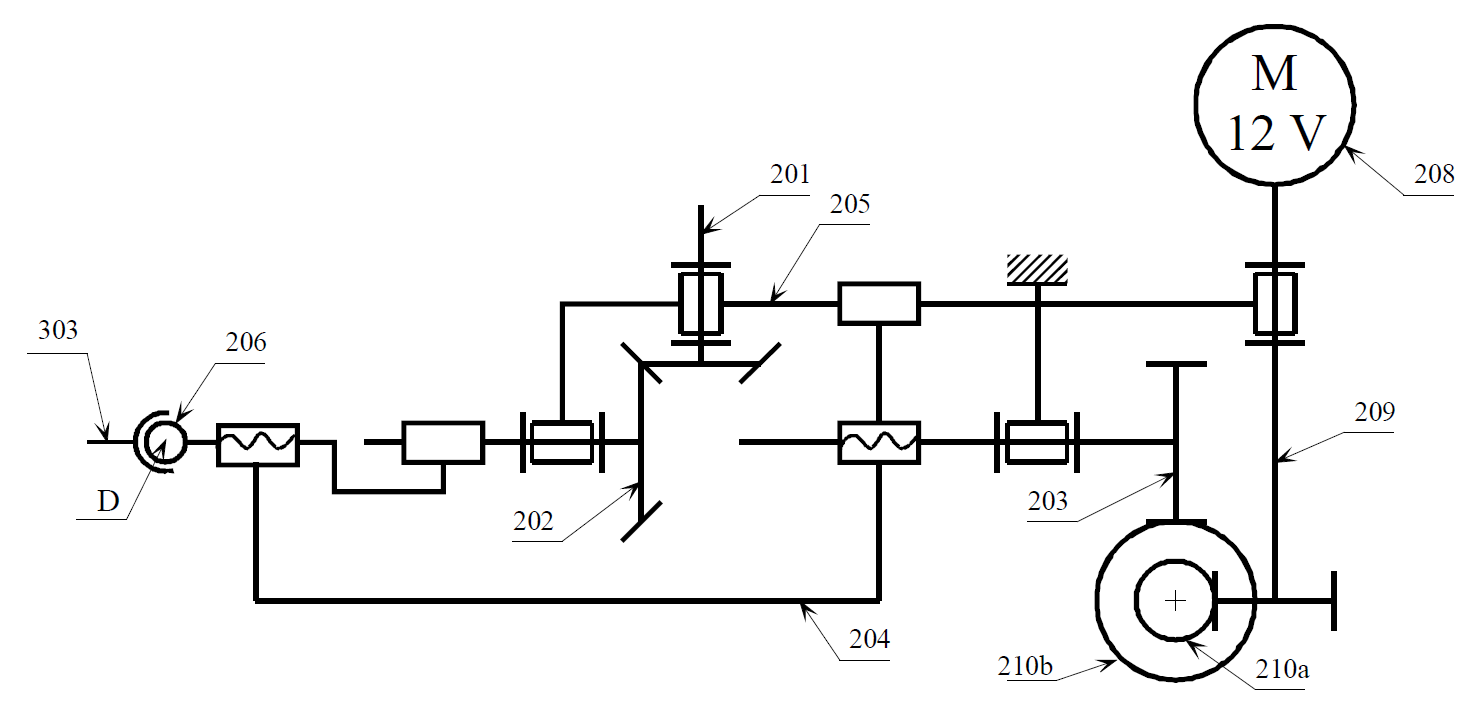
\includegraphics[width=0.8\linewidth]{img/phare10}
\end{center}

Réglage manuel

\begin{center}
  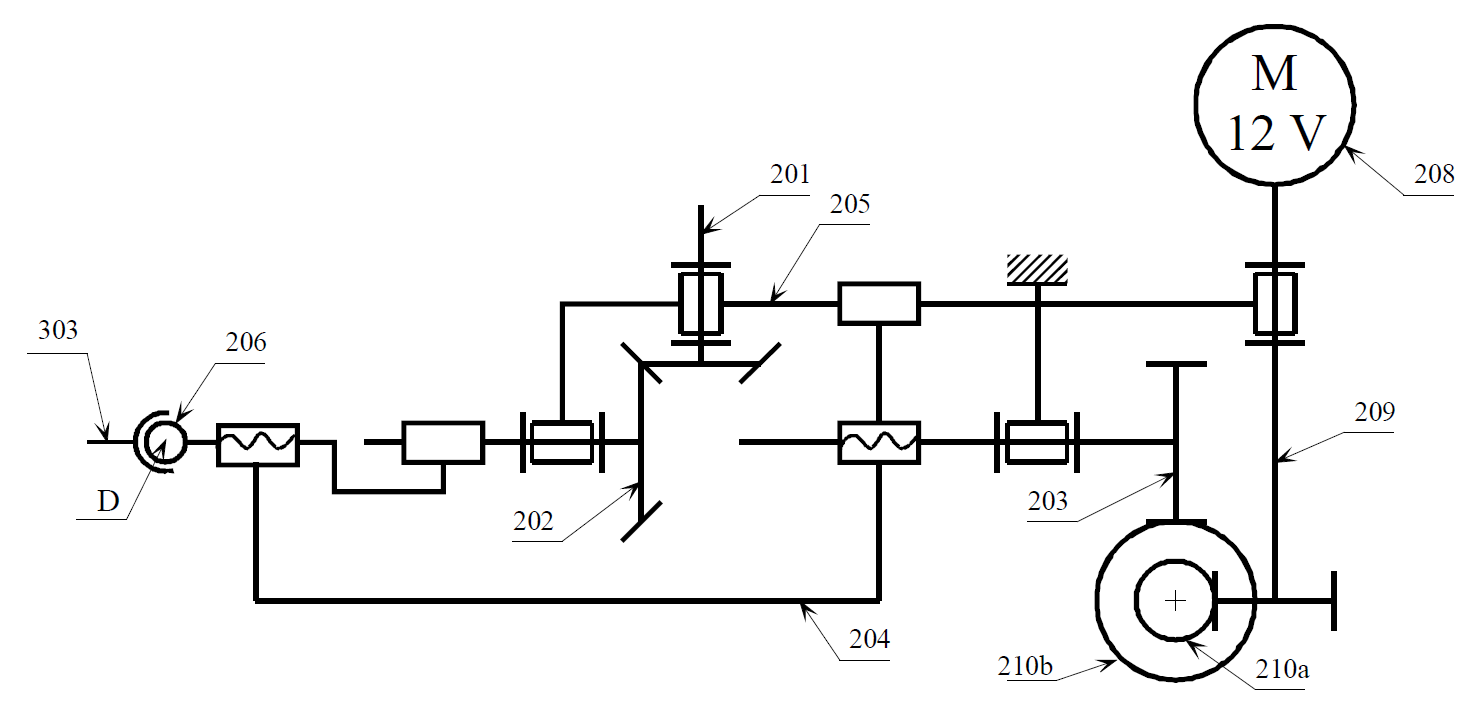
\includegraphics[width=0.8\linewidth]{img/phare10}
\end{center}

\newpage

\paragraph{Question 23:}

\begin{center}
  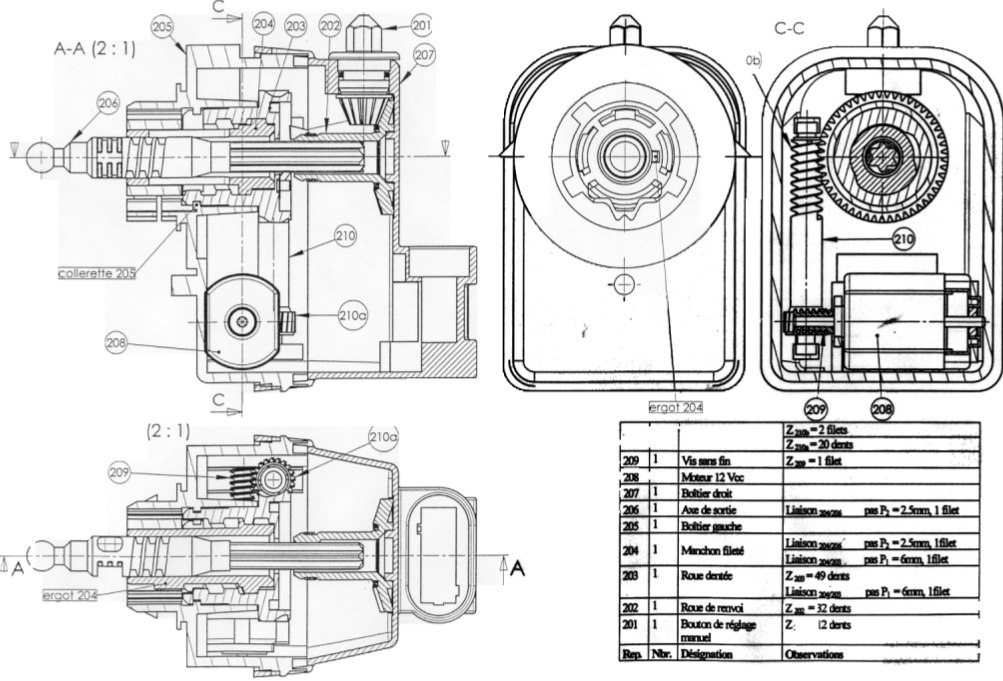
\includegraphics[width=\linewidth]{img/rep13}
\end{center}

\paragraph{Question 24:}

\reponse[6]

\paragraph{Question 25:}

\reponse[2]

\newpage

\paragraph{Questions 26 et 27:}

\begin{center}
  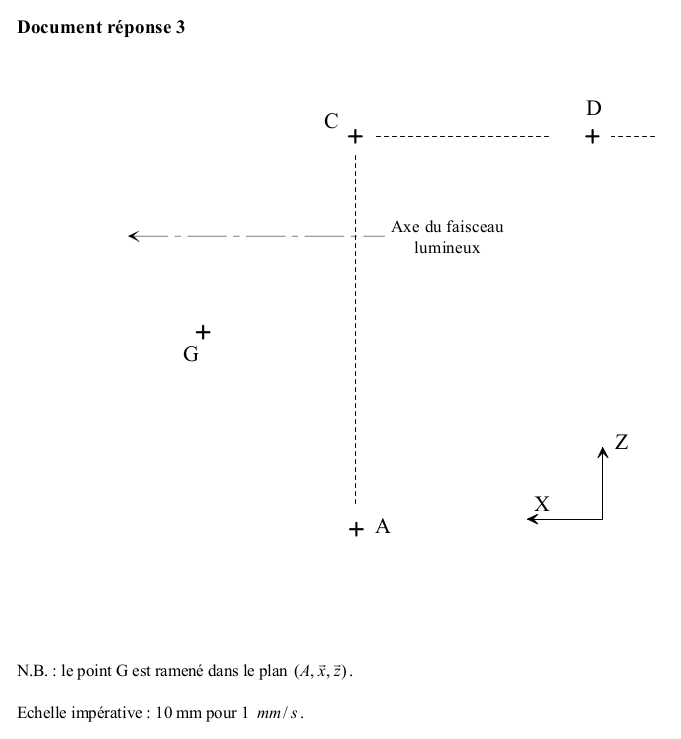
\includegraphics[width=0.8\linewidth]{img/rep14}
\end{center}

\reponse[2]

\cleardoublepage

\subsection{Robot préhenseur de pièces}

\paragraph{Question 28:}

\reponse[3]

\paragraph{Question 29:}

\reponse[3]

\paragraph{Question 30:}

\reponse[3]

\paragraph{Question 31:}

\begin{center}
\begin{minipage}{0.49\linewidth}
	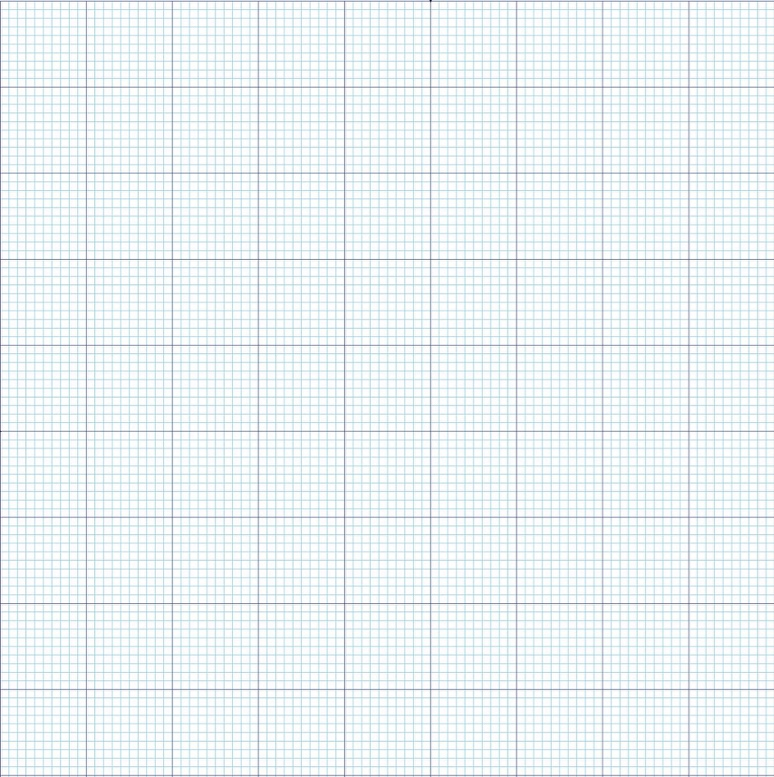
\includegraphics[width=\linewidth]{img/rep4}
\end{minipage}\hfill
\begin{minipage}{0.49\linewidth}
	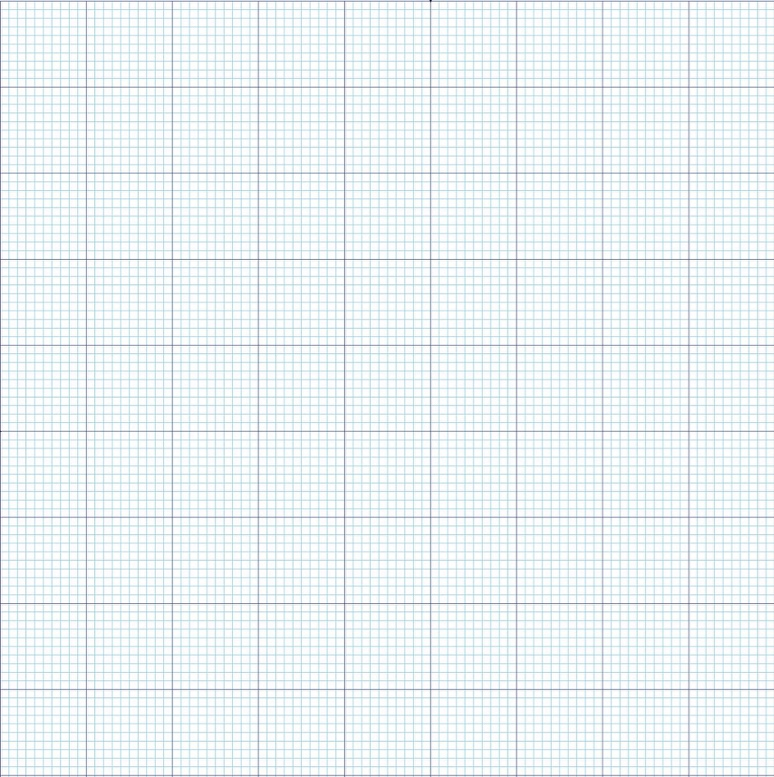
\includegraphics[width=\linewidth]{img/rep4}
\end{minipage}
\end{center}

\paragraph{Question 32:}

\reponse[3]

\paragraph{Question 33:}

\reponse[3]

\paragraph{Question 34:}

\reponse[6]

\paragraph{Question 35:}

\reponse[6]

\paragraph{Question 36:}

\reponse[5]

\cleardoublepage

\subsection{Torseur d'action mécanique transmissible par une liaison}

\paragraph{Question 37:}

\begin{center}
\begin{tabular}{|P{3cm}|P{3cm}|P{2cm}|P{2.5cm}|P{2.5cm}|}
\hline
Nom et description géométrique& Représentation 3D | 2D & Validité (axe ou direction) & Forme du torseur cinématique  (colonne) & Forme du torseur de l'action mécanique transmissible (colonne) \\
\hline
Pivot glissant d'axe $(O,\overrightarrow{x})$ & \vspace{0.5pt} 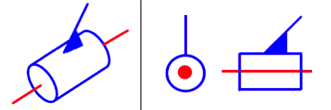
\includegraphics[width=3cm]{img/rep6} & Tout point A de l'axe $(O,\overrightarrow{x})$ & & \\
\hline
Sphère plan de point de contact O et de normale $\overrightarrow{z}$ & \vspace{0.5pt} 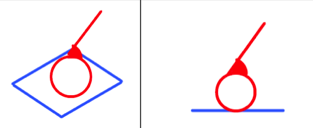
\includegraphics[width=3cm]{img/rep7} & Tout point A de la normale $(O,\overrightarrow{z})$ & & \\
\hline
Glissière de direction $\overrightarrow{x}$ & \vspace{0.5pt} 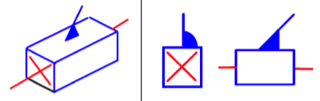
\includegraphics[width=3cm]{img/rep8} & Tout point A de l'espace & & \\
\hline
Pivot d'axe $(O,\overrightarrow{x})$ & \vspace{0.5pt} 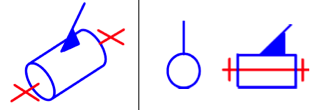
\includegraphics[width=3cm]{img/rep9} & Tout point A de l'axe $(O,\overrightarrow{x})$ & & \\
\hline
Appui plan de normale $\overrightarrow{z}$ & \vspace{0.5pt} 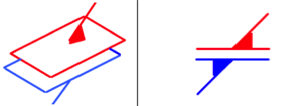
\includegraphics[width=3cm]{img/rep10} & Tout point A de l'espace & & \\
\hline
Linéaire rectiligne de ligne de contact $(O,\overrightarrow{x})$ et de normale $\overrightarrow{z}$& \vspace{0.5pt} 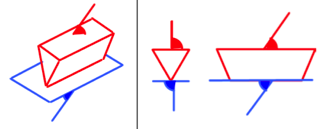
\includegraphics[width=3cm]{img/rep11} & Tout point A du plan $(O,\overrightarrow{x},\overrightarrow{z})$ & & \\
\hline
Hélicoïdale d'axe $(O,\overrightarrow{x})$ et de pas $p$ & \vspace{0.5pt} 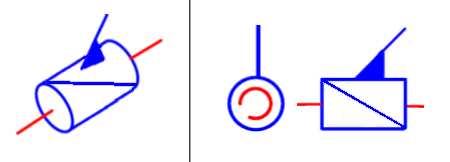
\includegraphics[width=3cm]{img/rep12} & Tout point A de l'axe $(O,\overrightarrow{x})$ & & \\
\hline
\end{tabular}
\end{center}

\reponse[3]

\newpage

\subsection{Assemblage vissé}

\paragraph{Question 38:}

\begin{center}
 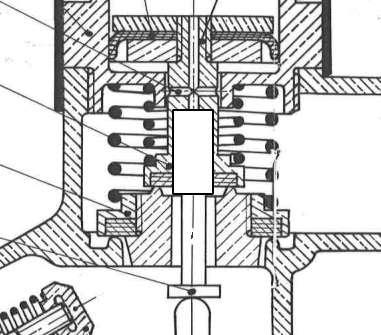
\includegraphics[width=0.8\linewidth]{img/zoom_lance}
\end{center}

\ifdef{\public}{\end{document}}{}

\newpage
\cleardoublepage

\pagestyle{correction}

\section{Correction}

\subsection{Correcteur de portée de phare}

\paragraph{Question 1:}

\begin{center}
  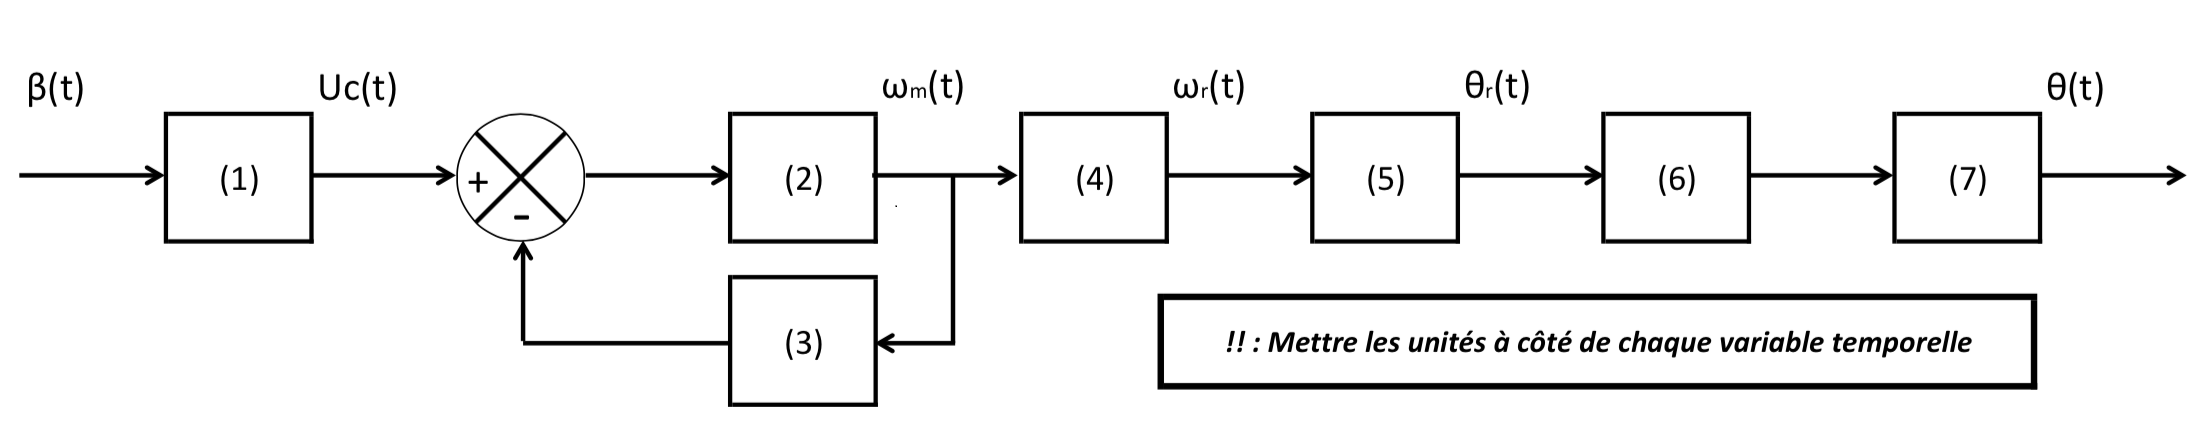
\includegraphics[width=0.8\linewidth]{img/rep1}

\begin{tabular}{|c|m{10cm}|}
\hline
 & Fonction \\
\hline
 (1) & Elaborer \\
  ~\ & $rad \rightarrow V$ \\
\hline
 (2) & Transformer NRJ élec>méca\\
  ~\ & $V \rightarrow rad.s^{-1}$ \\
\hline
 (3) & Acquérir\\
  ~\ & $rad.s^{-1} \rightarrow V$ \\
\hline
 (4) & Transmettre adapter (réducteur)\\
  ~\ & $rad.s^{-1} \rightarrow rad.s^{-1}$ \\
\hline
 (5) & Transformation vitesse>position (intégration)\\
  ~\ & $rad.s^{-1} \rightarrow rad$ \\
\hline
 (6) & Système vis-écrou\\
  ~\ & $rad \rightarrow mm$ \\
\hline
 (7) & Linéarisation (adapter)\\
  ~\ & $mm \rightarrow rad$\\
\hline
\end{tabular}
\end{center}

\paragraph{Question 2:}

On a $\frac{d\theta_r(t)}{dt}=\omega_r(t)$, CI nulles, théorème de la dérivation, $\Omega_r(p)=p.\theta_r(p)$.

\paragraph{Question 3:}

On a $x(t)=p_{vis}.\frac{\theta(t)}{2.\pi}$, CI nulles, donc $X(p)=p_{vis}.\frac{\Theta(P)}{2.\pi}$

\paragraph{Question 4:}

\begin{center}
  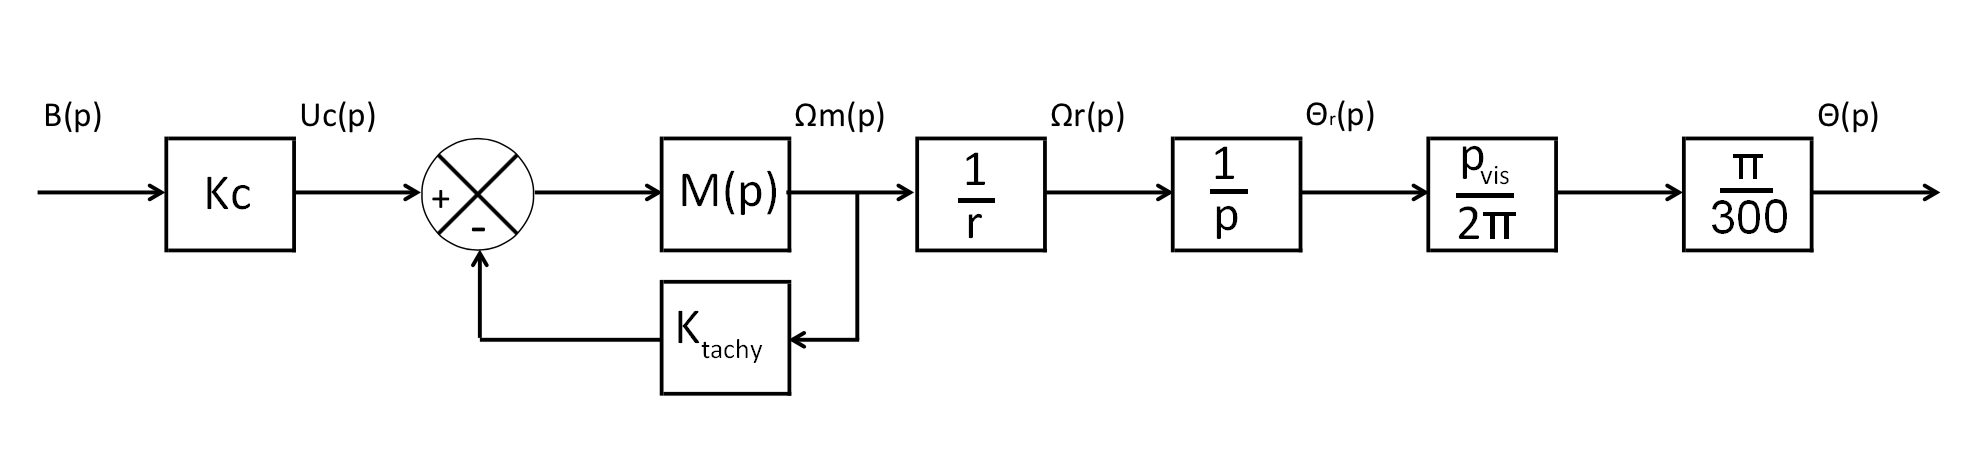
\includegraphics[width=0.9\linewidth]{img/rep2_cor}
\end{center}

\paragraph{Question 5:}

Tangente horizontale nulle à l'origine.

\paragraph{Question 6:}

En $+\infty$, l'asymptote vaut $300rad.sç{-1}$. $K.U_0=300$, donc $K=300$.

\paragraph{Question 7:}

$M(p)=\frac{K}{1+\frac{2.z}{\omega_n}.p+\frac{1}{\omega_n^2}.p^2}=\frac{K}{(1+T_1.p)(1+T_2.p)}$.

\paragraph{Question 8:}

Si $T_1>>T_2$, alors $M(p)=\frac{K}{1+T_1.p}$.

\paragraph{Question 9:}

$M(p)=\frac{K}{1+T_1.P}$, avec $K=300rad.s^{-1}$ et $T_1=0,05s$.

\paragraph{Question 10:}

Le temps de réponse à 5\% est le temps au bout duquel, pour une entrée en échelon, la réponse entre définitivement dans une bande de + ou - 5\% de la valeur définitive.

$t_{r5\%}=0,15s$.

\paragraph{Question 11:}

$t_{r5\%}\simeq3.T_1$, donc l'hypothèse de l'ordre 1 est vérifiée.

\paragraph{Question 12:}

$M'(p)=\frac{\Omega_m(p)}{U_c(p)}=\frac{\frac{K}{1+T_1.p}}{1+\frac{K_{tachy}.K}{1+T_1.p}}=\frac{K}{1+T_1.p+K_{tachy}.K}$

$M'(p)=\frac{K}{1+K_{tachy}.K}.\frac{1}{1+T_1.p}=-\infty$

\paragraph{Question 13:}

\begin{center}
	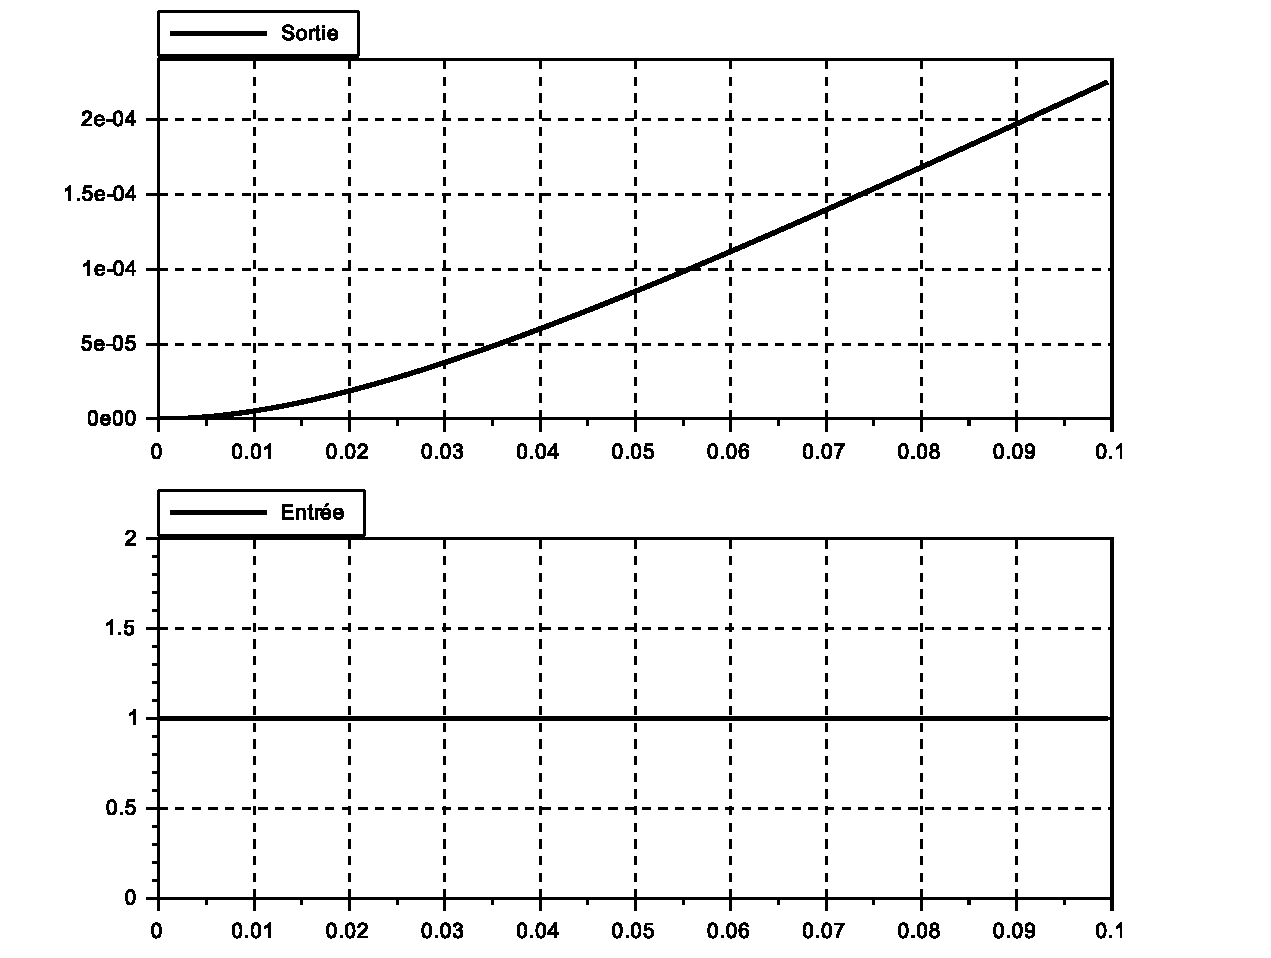
\includegraphics[width=\linewidth]{img/cor13}
\end{center}

\paragraph{Question 14:}

Théorème de la valeur finale.

$\epsilon_s=\lim\limits_{t \rightarrow +\infty} \beta(t)-\theta(t)=\lim\limits_{p \rightarrow 0+} p.(B(p)-\Theta(p))$, avec $B(p)=\frac{B_0}{p}$.

$\epsilon_s=\lim\limits_{p \rightarrow 0+} B_0.\left((1-\frac{0,003.K_c}{p.(1+0,025.p)}\right)=-\infty$.

\paragraph{Question 15:}
	
$H'(p)=\frac{\Theta(p)}{B(p)}=\frac{\Theta(p)}{U_c(p)}.\frac{U_c(p)}{B(p)}=\frac{\frac{K}{K_{pos}}}{1+\frac{1}{0,003.A.K_{pos}}.p+\frac{0,025}{0,003.A.K_{pos}}.p^2}=\frac{K}{K_{pos}}.\frac{1}{1+\frac{2.z}{\omega_n}.p+\frac{1}{\omega_n^2}.p^2}$

$K=\frac{K}{K_{pos}}$, $\omega_n=\frac{\sqrt{3.A.K_{pos}}}{5}$, $\xi=\frac{100}{\sqrt{3.A.K_{pos}}}$.

\paragraph{Question 16:}

$\epsilon_s=\lim\limits_{t \rightarrow +\infty} \beta(t)-\theta(t)=\lim\limits_{p \rightarrow 0+} p.(B(p)-\Theta(p))=B_0.\left(1-\frac{K}{K_{pos}}\right)$.


\paragraph{Question 17:}

Le retour tachymétrique a permis de borner l'écart statique du système. Cela revient à mettre en place un asservissement.

\paragraph{Question 18:}

Le système est le plus rapide si $\xi=0,69=\frac{\sqrt{2}}{2}$, donc $\frac{\sqrt{2}}{2}=\frac{100}{\sqrt{3.A.K_{pos}}}$, donc $A.K_{pos}=\frac{20000}{3}=6666$.

\paragraph{Question 19:}

$t_{R,5\%}.\omega_n=3$, donc $t_{R,5\%}=\frac{3}{\omega_n}=\frac{3}{28}=0,1s$.

\paragraph{Question 20:}

Par lecture, $X_1=0,05$, c'est le point de départ du calcul du $\xi$ le plus rapide.

\paragraph{Question 21:}

Le système est le plus rapide sans dépassement si $\xi=1$, donc $1=\frac{100}{\sqrt{3.A.K_{pos}}}$, donc $A.K_{pos}=\frac{10000}{3}=3333$.

\paragraph{Question 22:}

~\

Réglage motorisé

\begin{center}
  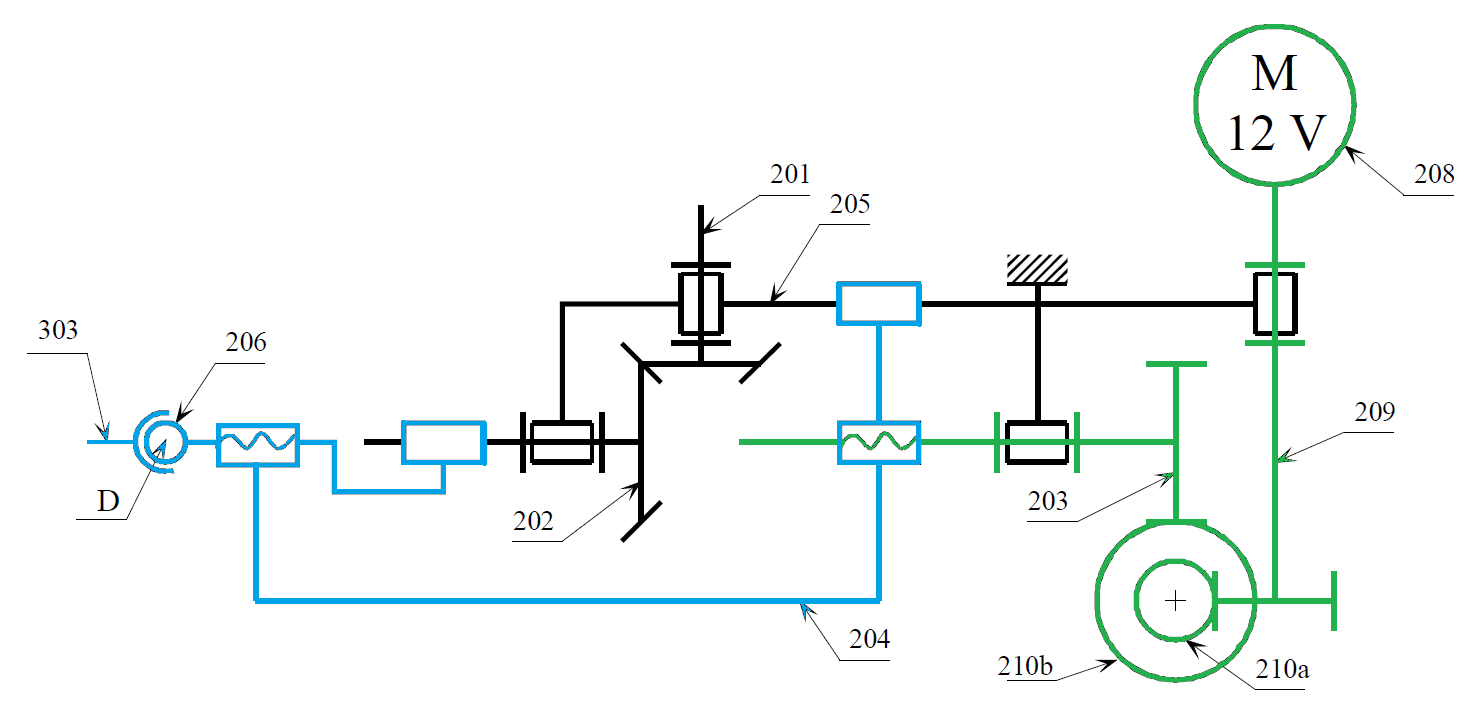
\includegraphics[width=0.8\linewidth]{img/phare101_cor}
\end{center}

Réglage manuel

\begin{center}
  \includegraphics[width=0.8\linewidth]{img/phare102_cor}
\end{center}

\newpage

\paragraph{Question 23:}

\begin{center}
  \includegraphics[width=\linewidth]{img/rep13_cor}
\end{center}

\paragraph{Question 24:}

$\left\{V_{304/302}\right\}=\left\{
\begin{array}{c c}
\omega x_{304/302} & 0 \\
\omega y_{304/302} & 0 \\
\omega z_{304/302} & 0 \\
\end{array}
\right\}_B$

$\left\{V_{302/301}\right\}=\left\{
\begin{array}{c c}
0 & 0 \\
0 & Vy_{302/301} \\
0 & 0 \\
\end{array}
\right\}_B$

Donc,

$\left\{V_{304/302}\right\}=\left\{
\begin{array}{c c}
\omega x_{304/302} & 0 \\
\omega y_{304/302} & Vy_{302/301} \\
\omega z_{304/302} & 0 \\
\end{array}
\right\}_B$

Il s'agit bien d'une liaison linéaire annulaire d'axe $(B,\overrightarrow{y})$.

\paragraph{Question 25:}

La liaison globale est une liaison pivot d'axe $(B,\overrightarrow{y})$.

\paragraph{Questions 26 et 27:}

\begin{center}
  \includegraphics[width=0.6\linewidth]{img/rep141_cor}
\end{center}

\begin{center}
  \includegraphics[width=0.6\linewidth]{img/rep142_cor}
\end{center}

\subsection{Robot préhenseur de pièces}

\paragraph{Question 28:}

Lorsque $\Theta(p)=\Theta_c(p)$, $\epsilon(p)=$, donc $\Theta_c(p).K_1-\Theta(p).K_7=0$, donc $K_1=K_7$.
\paragraph{Question 29:}

Théorème de la dérivée finale et conditions initiales nulles, donc:

$U_m(p)=k_e.\Omega(p)+\frac{R.J}{k_m}.p.\Omega(p)$,

$H_3(p)=\frac{\Omega(p)}{U_m(p)}=\frac{\frac{1}{k_e}}{1+\frac{R.J}{k_e.k_m}.p}$, ainsi, $\tau_3=\frac{R.J}{k_e.k_m}$.

\paragraph{Question 30:}

$\omega_m(t)=K.U_0.(1-e^{-\frac{t}{\tau_3}})$, avec $K=\frac{1}{k_e}$ et $\tau_3=\frac{R.J}{k_e.k_m}$.

\paragraph{Question 31:}

\begin{center}
	\includegraphics[width=0.8\linewidth]{img/cor31}
\end{center}

\paragraph{Question 32:}

D'après le théorème de l'intégrale, $H_4(p)=\frac{1}{p}$.

\paragraph{Question 33:}

$H(p)=\dfrac{1}{1+\frac{1}{K_{corr}.K_3.K_5.K_6.K_7}.p+\frac{\tau_3}{K_{corr}.K_3.K_5.K_6.K_7}.p^2}$

Ainsi, $K_0=1$, $\omega_n=\sqrt{\frac{K_{corr}.K_3.K_5.K_6.K_7}{\tau_3}}$ et $\xi=\frac{1}{2}.\sqrt{\frac{1}{\tau_3.K_{corr}.K_3.K_5.K_6.K_7}}$.

\paragraph{Question 34:}

On lit sur la courbe:
\begin{itemize}
 \item $K_0.E_0=1$, avec $E_0=1$ donc $K_0=1$,
 \item $D_1\simeq0,5$, donc $z\simeq 0,22$,
 \item $t_{R,5\%}\simeq 0,28s$, or $z=0,22$, donc $t_{R,5\%}.\omega_n=15$, donc $\omega_n=53,5rad.s^{-1}$.
\end{itemize}

En traçant ce résultat sur scilab, on obtient la courbe suivante:
\begin{center}
 \includegraphics[width=0.6\linewidth]{img/cor34}
\end{center}

\paragraph{Question 35:}

Le temps de réponse peut être lu sur la figure, il s'agit de l'instant à partir duquel la courbe reste dans la plage $0,95-1,05$ $(+/-5\%)$, ici, le temps de réponse est de 0,28s.

\paragraph{Question 36:}

Le cahier des charges n'est pas respecté car $0,28s>0,2s$.

\newpage

\subsection{Torseur d'action mécanique transmissible par une liaison}

\paragraph{Question 37:}

\begin{center}
\begin{tabular}{|P{2.5cm}|P{3cm}|P{2cm}|P{3cm}|P{3cm}|}
\hline
Nom et description géométrique& Représentation 3D | 2D & Validité (axe ou direction) & Forme du torseur cinématique  (colonne) & Forme du torseur de l'action mécanique transmissible (colonne) \\
\hline
Pivot glissant d'axe $(O,\overrightarrow{x})$ & \vspace{0.5pt} \includegraphics[width=3cm]{img/rep6} & Tout point A de l'axe $(O,\overrightarrow{x})$ & $\left\{
\begin{matrix}
 \omega x_{ij} & Vx_{A,ij} \\
 0 & 0 \\
 0 & 0 
\end{matrix}
\right \}_{A}$ & 
$\left\{\begin{matrix}
 0 & 0 \\
 Y_{ij} & {M }_{A,ij} \\
 Z_{ij} & {N }_{A,ij} 
\end{matrix}
\right \}_{A} $ \\
\hline
Sphère plan de point de contact O et de normale $\overrightarrow{z}$ & \vspace{0.5pt} \includegraphics[width=3cm]{img/rep7} & Tout point A de la normale $(O,\overrightarrow{z})$ & $\left\{
\begin{matrix}
 \omega x_{ij} & Vx_{A,ij} \\
 \omega y_{ij} & Vy_{A,ij} \\
 \omega z_{ij} & 0 
\end{matrix}
\right \}_{A}$ & 
$\left\{\begin{matrix}
 0 & 0 \\
 0 & 0 \\
 Z_{ij} & 0
\end{matrix}
\right \}_{A} $ \\
\hline
Glissière de direction $\overrightarrow{x}$ & \vspace{0.5pt} \includegraphics[width=3cm]{img/rep8} & Tout point A de l'espace & $\left\{
\begin{matrix}
 0 & Vx_{A,ij} \\
 0 & 0 \\
 0 & 0
\end{matrix}
\right \}_{A}$ & 
$\left\{\begin{matrix}
 0 & {L }_{A,ij} \\
 Y_{ij} & {M }_{A,ij} \\
 Z_{ij} & {N }_{A,ij} 
\end{matrix}
\right \}_{A} $ \\
\hline
Pivot d'axe $(O,\overrightarrow{x})$ & \vspace{0.5pt} \includegraphics[width=3cm]{img/rep9} & Tout point A de l'axe $(O,\overrightarrow{x})$ & $\left\{
\begin{matrix}
 \omega x_{ij} & 0 \\
 0 & 0 \\
 0 & 0 
 \end{matrix}
\right \}_{A}$ & 
$\left\{\begin{matrix}
 X_{ij} &0 \\
 Y_{ij} & {M }_{A,ij} \\
 Z_{ij} & {N }_{A,ij} 
\end{matrix}
\right \}_{A} $ \\
\hline
Appui plan de normale $\overrightarrow{z}$ & \vspace{0.5pt} \includegraphics[width=3cm]{img/rep10} & Tout point A de l'espace & $\left\{
\begin{matrix}
 0 & Vx_{A,ij} \\
 0 & Vy_{A,ij} \\
 \omega z_{ij} & 0 
\end{matrix}
\right \}_{A}$ & 
$\left\{\begin{matrix}
 0 & {L }_{A,ij} \\
 0 & {M }_{A,ij} \\
 Z_{ij} & 0 
\end{matrix}
\right \}_{A} $ \\
\hline
Linéaire rectiligne de ligne de contact $(O,\overrightarrow{x})$ et de normale $\overrightarrow{z}$& \vspace{0.5pt} \includegraphics[width=3cm]{img/rep11} & Tout point A du plan $(O,\overrightarrow{x},\overrightarrow{z})$ & $\left\{
\begin{matrix}
 \omega x_{ij} & Vx_{A,ij} \\
 0 & Vy_{A,ij} \\
 \omega z_{ij} & 0 
\end{matrix}
\right \}_{A}$ & 
$\left\{\begin{matrix}
 0 & 0 \\
 0 & {M }_{A,ij} \\
 Z_{ij} & 0 
\end{matrix}
\right \}_{A} $ \\
\hline
Hélicoïdale d'axe $(O,\overrightarrow{x})$ et de pas $p$ & \vspace{0.5pt} \includegraphics[width=3cm]{img/rep12} & Tout point A de l'axe $(O,\overrightarrow{x})$ & $\left\{
\begin{matrix}
 \omega x_{ij} & Vx_{P,ij} \\
 0 & 0 \\
 0 & 0 
\end{matrix}
\right \}_{A}$ & 
$\left\{\begin{matrix}
 X_{ij} & {L }_{P,ij} \\
 Y_{ij} & {M }_{P,ij} \\
 Z_{ij} & {N }_{P,ij} 
\end{matrix}
\right \}_{A} $ \\
\hline
\end{tabular}
\end{center}

Avec pour l'hélicoïdale: $Vx_{P,ij}=\frac{p}{2.\pi}.\omega x_{ij}$ et ${L }_{P,ij}=\frac{p}{2.\pi}.X_{ij}$.

\newpage
\subsection{Assemblage vissé}

\paragraph{Question 38:}

\begin{center}
 \includegraphics[width=0.8\linewidth]{img/cor38}
\end{center}


\end{document}

